\documentclass{article}
\usepackage{graphicx}
\usepackage{color}
\usepackage{fullpage}
\usepackage[colorlinks=false]{hyperref}

\RequirePackage{natbib}

\begin{document}

\title{Data Visualization and Statistical Graphics in Big Data Analysis}%: What are the modern successors to John W. Tukey's pencil and paper, and mainframe computer, tools?}
\author{Dianne Cook, Department of Statistics, Iowa State University\\
Eun-Kyung Lee, Department of Statistics, Ewha Womans University\\
Mahbubul Majumder, University of Nebraska-Omaha}
%\date{These are the thoughts that I have for pulling together the article on Visualization of Big Data for the Annual Reviews. }
%\date{}
\maketitle

\section{Introduction}

In the 1970s J. W. Tukey introduced the world to exploratory data analysis (EDA). Data visualization was a major component of this area, and Tukey made substantial contributions to statistical graphics. (A good summary of his contributions can be found in \citet{stuetzlefriedman2002}.) His philosophy was that good pictures of data can reveal what we never expected to see. His pencil and paper method, the stem-and-leaf plot, is universally taught in introductory statistics, and the fruits of his experiments in plotting high-dimensional data in the PRIM-9 system can be found in today's data visualization software. Even such widely visible systems such as GapMinder (\url{http://www.gapminder.org}) and BabyNameVoyager (\url{http://www.babynamewizard.com/}) owe some credit to interactive graphics that arose in the first years of EDA research.

It's surprising that the stem-and-leaf plot has persisted in the classroom to present day. The pencil paper methods were essential to the 1970s because access to the technology to do interactive graphics was limited. Today there is almost universal access to technology for data analysis and little need for hand-sketching numbers. Today's EDA is very much about harnessing good computer-generated plots of data. Tukey was fortunate enough to have access to state-of-the-art technology, and was also an early advocate of harnessing technology for data analysis. Forty-five years ago he foresaw today's technological big data world and just how important computational tools would be for statistical analysis and how good utilization of technology can attract the best young talent to the field.

 %Some of his famous quotes point to the reasons for the importance of statistical graphics:

%\begin{quote}
%{\em Good pictures of data ``force the unexpected upon us.'' } (J. W. Tukey)
%\end{quote}

%\noindent and he was also :

%\begin{quote}
%{\em ``Today, software and hardware together provide far more powerful factories than most statisticians realize, factories that many of
%today's most able young people find exciting and worth learning about on their own''}
%\end{quote}

It is important to realize that EDA did not entirely arise in a vacuum. Applied statistical practice has always utilized data plots prior to modeling to check assumptions and for post-model assessment of the fit. \citet{CH90} make this very clear:

\begin{quote}
{\em ``The first thing to do with data is to look at them.... usually
means tabulating and plotting the data in many different ways to `see
what's going on'. With the wide availability of computer packages and
graphics nowadays there is no excuse for ducking the labour of this
preliminary phase, and it may save some red faces later.''}
\end{quote}

\noindent Big data provides new challenges for data visualization. Being able, and knowing how to, make good data plots is an indispensable component of wrangling with big data. The term ``big data'' means something different depending who you listen to, read, or chat with. The working definition for this article is not entirely to do with size of the data in terms of variables, or samples, but also the complexity. It may be data that has hundreds of variables, stored in many related tables, a large database that has been collected and perhaps neglected for many years, repositories of emails, health records from machines in almost every doctor's office that automatically files information, communications networks from social media, scores from tests administered to our youth across the globe, humongous quantities of data simulated from global climate models to assess the impact of climate change, or new business data being collected and stored in new systems like hadoop. We are interested in data that potentially informs  us about our world, to learn how to be more efficient in business operations or in delivering health care, what statistics we need improve to get our tennis game to the level of a champion, or who are the key people that bind a social network into a cohesive group.

John Tukey's EDA, and the tools for plotting your data are all around us today. Knowing how to effectively leverage visualization is a fundamental skill of today's society. New methods and software have made this easy and accessible for most people today. Big data, open data and open source software, makes this a golden age for data visualization.

{\color[rgb]{1,0,0} In classical statistical inference and experimental studies, the role of data is just to prove the conjecture. In this case the distribution of test statistic is preferably derived theoretically. Data is used to obtain empirical distribution when it is not possible though. In any case, the role of data is passive and has very specific purpose. We can illustrate this by an example. In a situation where researchers want to test the population mean being equal to a certain value, they don't need the data to find the distribution of test statistic as long as some assumptions are met. Data is used only to find the evidence for or against the hypothesis. The formation of hypothesis as well as the derivation of test methods do not require data. It is only needed to finally make the decision.

However, the advent of big data has changed the classical way of thinking. A researcher with enormous amount of data does not necessarily have a well defined hypothesis in mind let alone having test methods. The challenge is to explore data and discover hidden value in the data which may later lead to more formal hypothesis and classical methods to test that.Thus big data turns the role of data more active where data comes first more often. This essentially requires adopting EDA and visualization as very earlier steps for big data analysis. The added advantage of visualization is that it can be used to perform statistical test using visual statistical inference, a method that does not require to satisfy hard-core classical style assumptions allowing making inferential decisions on the fly while doing EDA.}

This paper has three components: (1) Contemporary illustrations of the usefulness of data visualization for understanding data, (2) a review of the literature on methodology for big data visualization, and (3) a review of technological advances that make big data visualization possible. Inevitably, the review cannot be entirely comprehensive, and we ask for the reader's leniency upfront if we do not name all the people and work that have made important contributions, but we hope that our coverage points to a broad selection of advances that will entice the reader to use these as a starting point to dig deeper and independently discover more interesting developments.

\section{Illustrations of Visualization for Understanding Data}

\subsection{How to Win a Data Mining Challenge!}

Two stories from 2014 point to the use of graphics from successful data mining teams: the key to their model winning the competition was the data pre-processing involving a lot of data plots that helped them to understand what they were working with, and problems with the data that needed to be addressed before being able to make effective models. This is important for big data, how to effectively clean, transform and pre-process large complex data sets. Visualization plays a key role. This is just as important for big data as it was for John Tukey's days, and the technology has radically changed.

\subsubsection{Kaggle Health Heritage Prize}

In April, 2011 Kaggle posted the details of the Heritage Health Prize ``Improve Healthcare, Win \$3,000,000''.  Dr Phil Brierley was part of the three person team that won the first two milestone awards of \$230,000, and combined forces with another team to win the final prize of \$500,000. This competition is an example of big data challenges of today: large amounts of data on hospital admissions being used to develop models to improve the efficiency of healthcare spending. In interviews post-prize, there are echoes of Tukey's long ago words:

\begin{quote}
{\em ``In many of the analytics problems I have been involved in, the problem you end up dealing with is not the one you initially were briefed to solve.
These new problems are always discovered by visualising the data in some way and spotting curious patterns.'' }\url{http://www.anotherdataminingblog.blogspot.co.uk/2011/12/whats-going-on-here.html}
\end{quote}

\begin{figure*}[htp]
\centerline{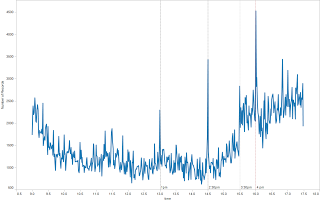
\includegraphics[width=4in]{images/shockeventtimings.png}}
\caption{Times of ``liquidity shocks'' in data from the London Stock Exchange. (Reprinted with permission from \url{http://www.anotherdataminingblog.blogspot.co.uk/2011/12/whats-going-on-here.html}.)}
\label{liqshock}
\end{figure*}

Here is an example from Dr Brierley's blog, that illustrates a algorithmic trading challenge. Figure \ref{liqshock} shows a plot made of timing of ``liquidity shocks'' in data from the London Stock Exchange -- yes, this is a really simple plot, but it tells us a lot about the data, which is:

\begin{quote}
{\em ``Now it is quite clear there is something going on at 1pm, 2:30pm, after 3:30pm and at 4pm.

Interestingly these spikes are only evident when all commodities are looked at together, they are not as obvious in any individual commodity.

My first question if I was solving a business problem would be to return to the business to get more insight in what was going on here. My initial thoughts were lunch breaks and the opening times of other Stock Exchanges around the world - as 3:30pm London time could be around opening time in New York.

Understanding the cause of these peaks is important as you would expect the reaction to them (the problem to solve) to be a function of the cause.

If we did discover it was the opening times of other exchanges, then I would ask for extra information like the specific dates, so I could calculate when these peaks would occur in the future when the clocks changed. We do not have this information at the current time, or even the day of the week (it can be inferred but not accurately as there will be public holidays when the exchanges are closed)

As it stands any models built could potentially fail on the leaderboard (or real life) data as our model might think 2:30pm is a special time, whereas really it is when another exchange opens, or when people come back from lunch. We need this causal information rather than just dealing with the effect - time differences change - lunch breaks may change.

The current competition data is potentially lacking the full information required to build a model that is as robust as possible over time.'' }
\end{quote}

\subsubsection{Data Mining Cup}

Each year Prudsys AG  challenges students with  the Data Mining Cup competition. In 2014, the problem was announced to student team on April 2, and students needed to have their final entry by May 14. The student teams had six weeks to develop a solution for a data mining problem on the topic of optimal return prognosis. More specifically, the goal was to use an online shop? historical purchase data to come up with a model for new orders that would calculate the probability of a purchase leading to a return. In this year's competition, a team of students (Guillermo Basulto-Elias (statistics), Fan Cao (statistics), Xiaoyue Cheng (statistics), Marius Dragomiroiu (computer science), Jessica Hicks (bioinformatics and computational biology), Cory Lanker (statistics), Ian Mouzon (statistics), Lanfeng Pan (statistics) and Xin Yin (bioinformatics and computational biology/statistics) from Iowa State University was the first north American team to win. A key component of that win was the pre-processing of the data, that utilized substantial graphics to learn about their data, and inform their modeling.

Figure \ref{DMC1} shows one plot used early by the ISU DMC team, to examine return rates by time and product. Yellow indicates the ordered items were kept, blue means they were returned and pink are items to be predicted. Yes, it is a really ugly plot!!! However, it is very informative: Two major structures are immediately visible, new product introductions in July 2012 and January 2013. The most important feature, though, is that new data to be predicted was in the third season of the time period, and this information was crucial to construct good training and test sets for model building.

\begin{figure*}[htp]
\centerline{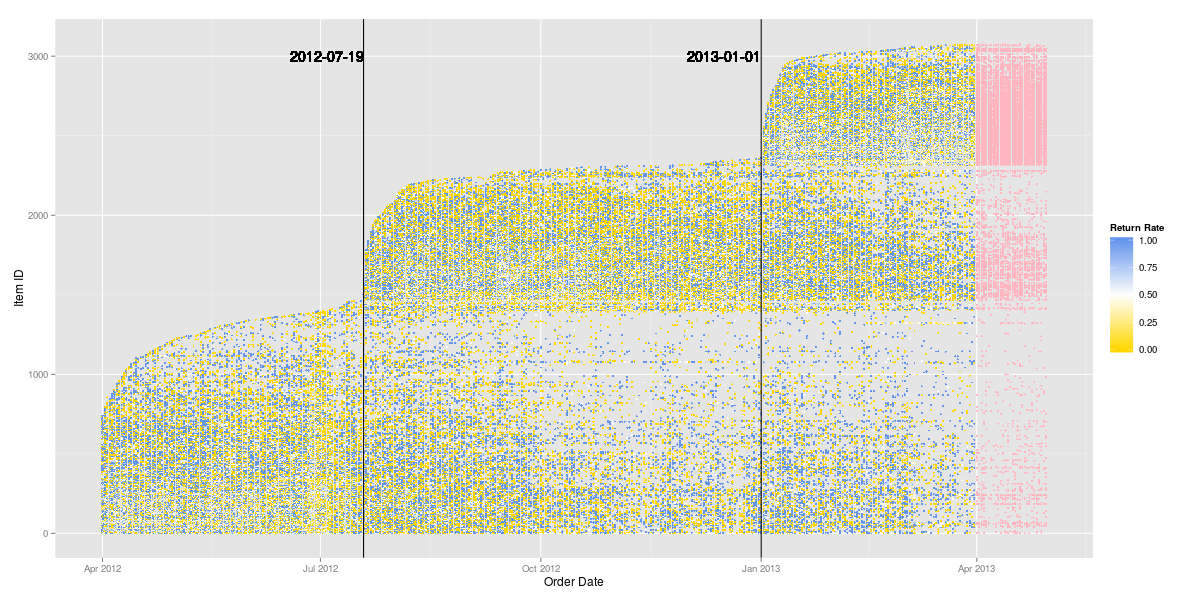
\includegraphics[width=7in]{images/orderDate_itemID.png}}
\caption{One of the preliminary plots made by the ISU DMC team. Item ID is plotted against order date, colored by return rate. The students learned that the data to be predicted (pink) did not look like the training data provided for building a model (blue/yellow).}
\label{DMC1}
\end{figure*}

\subsection{Visualization is NOT Prediction}

.... and it is beneficial in its own right. In this section, we will describe examples of visualization being used in the process of analyzing big data sets, partially from our own work and two examples from published work. What we learn from plots is different from that of modeling and prediction.

%For big data, there are possibly many, many, many things that might be learned. There are likely many facets to the data. It is important to note that exploring big data visually is typically generating, not testing, hypotheses.

\subsubsection{OECD PISA}

The Programme for International Student Assessment (PISA) is a triennial survey conducted by the Organization for Economic Cooperation and Development (OECD) with a rotating emphasis on one of mathematics, reading, or science. In 2012, the emphasis was on mathematics. The data was made available by the OECD as part of a data challenge for the useR! 2014 conference. Entries to the competition can be found at http://beta.icm.edu.pl/PISAcontest/.

This data is big because there is a lot of information collected in addition to the test scores. In the student table there are records for about 500,000 students from 65 different countries, and 635 variables. The variables include information about gender, language, household possessions attitude to math, use of the internet, many different aspects of their lives. The parent table has 143 variables from 100,000 parent-completed surveys providing information about the students households, such as if both parents are in the home or if its a foster home, parents occupations, how the child's school was selected. The school table contains survey results completed by 18,000 school principals producing 291 variables. These items include information about numbers of teachers, supply shortages, teacher turnover, educational background of teachers, streaming of classes. There are many different questions that we might try to answer with this data. After the magnitude of the data was determined, by making quick counts of each of the tables provided, and examining the data dictionaries, our group hashed out possible questions and expectations of what associations we might see in the data.

One issue that we were interested in was about the gender gap between boys and girls in math. We hear about this in the media frequently, and we were interested to see if evidence of the gap was present in this multinational test data. To examine this question we calculated the difference between the mean math test scores for boys and girls in each of the countries, and plotted it. Sample weights were utilized in calculating the averages. The result is shown in Figure \ref{OECD-gender}. The absence of a universal math gap runs counter to the popular press. This data represents an observational study, and so it can only inform us about association. To understand some potential reasons why the gap does not exist should involve additional investigations into the samples used in each country. One quick check reveals that it cannot be explained by differing proportions of boys and girls being tested: these are roughly the same in all countries, so the math gap in favor of girls in some countries is not due to just a few top girls being tested.

This data is abounding with information ripe for exploration. We can learn about many associations between demographic factors and educational achievement about countries across the globe. These could be mined to form the basis for follow-up experimental studies. Visualization provides an excellent way to mine these associations, across the different categorical levels.

\begin{figure*}[tp]
\centerline{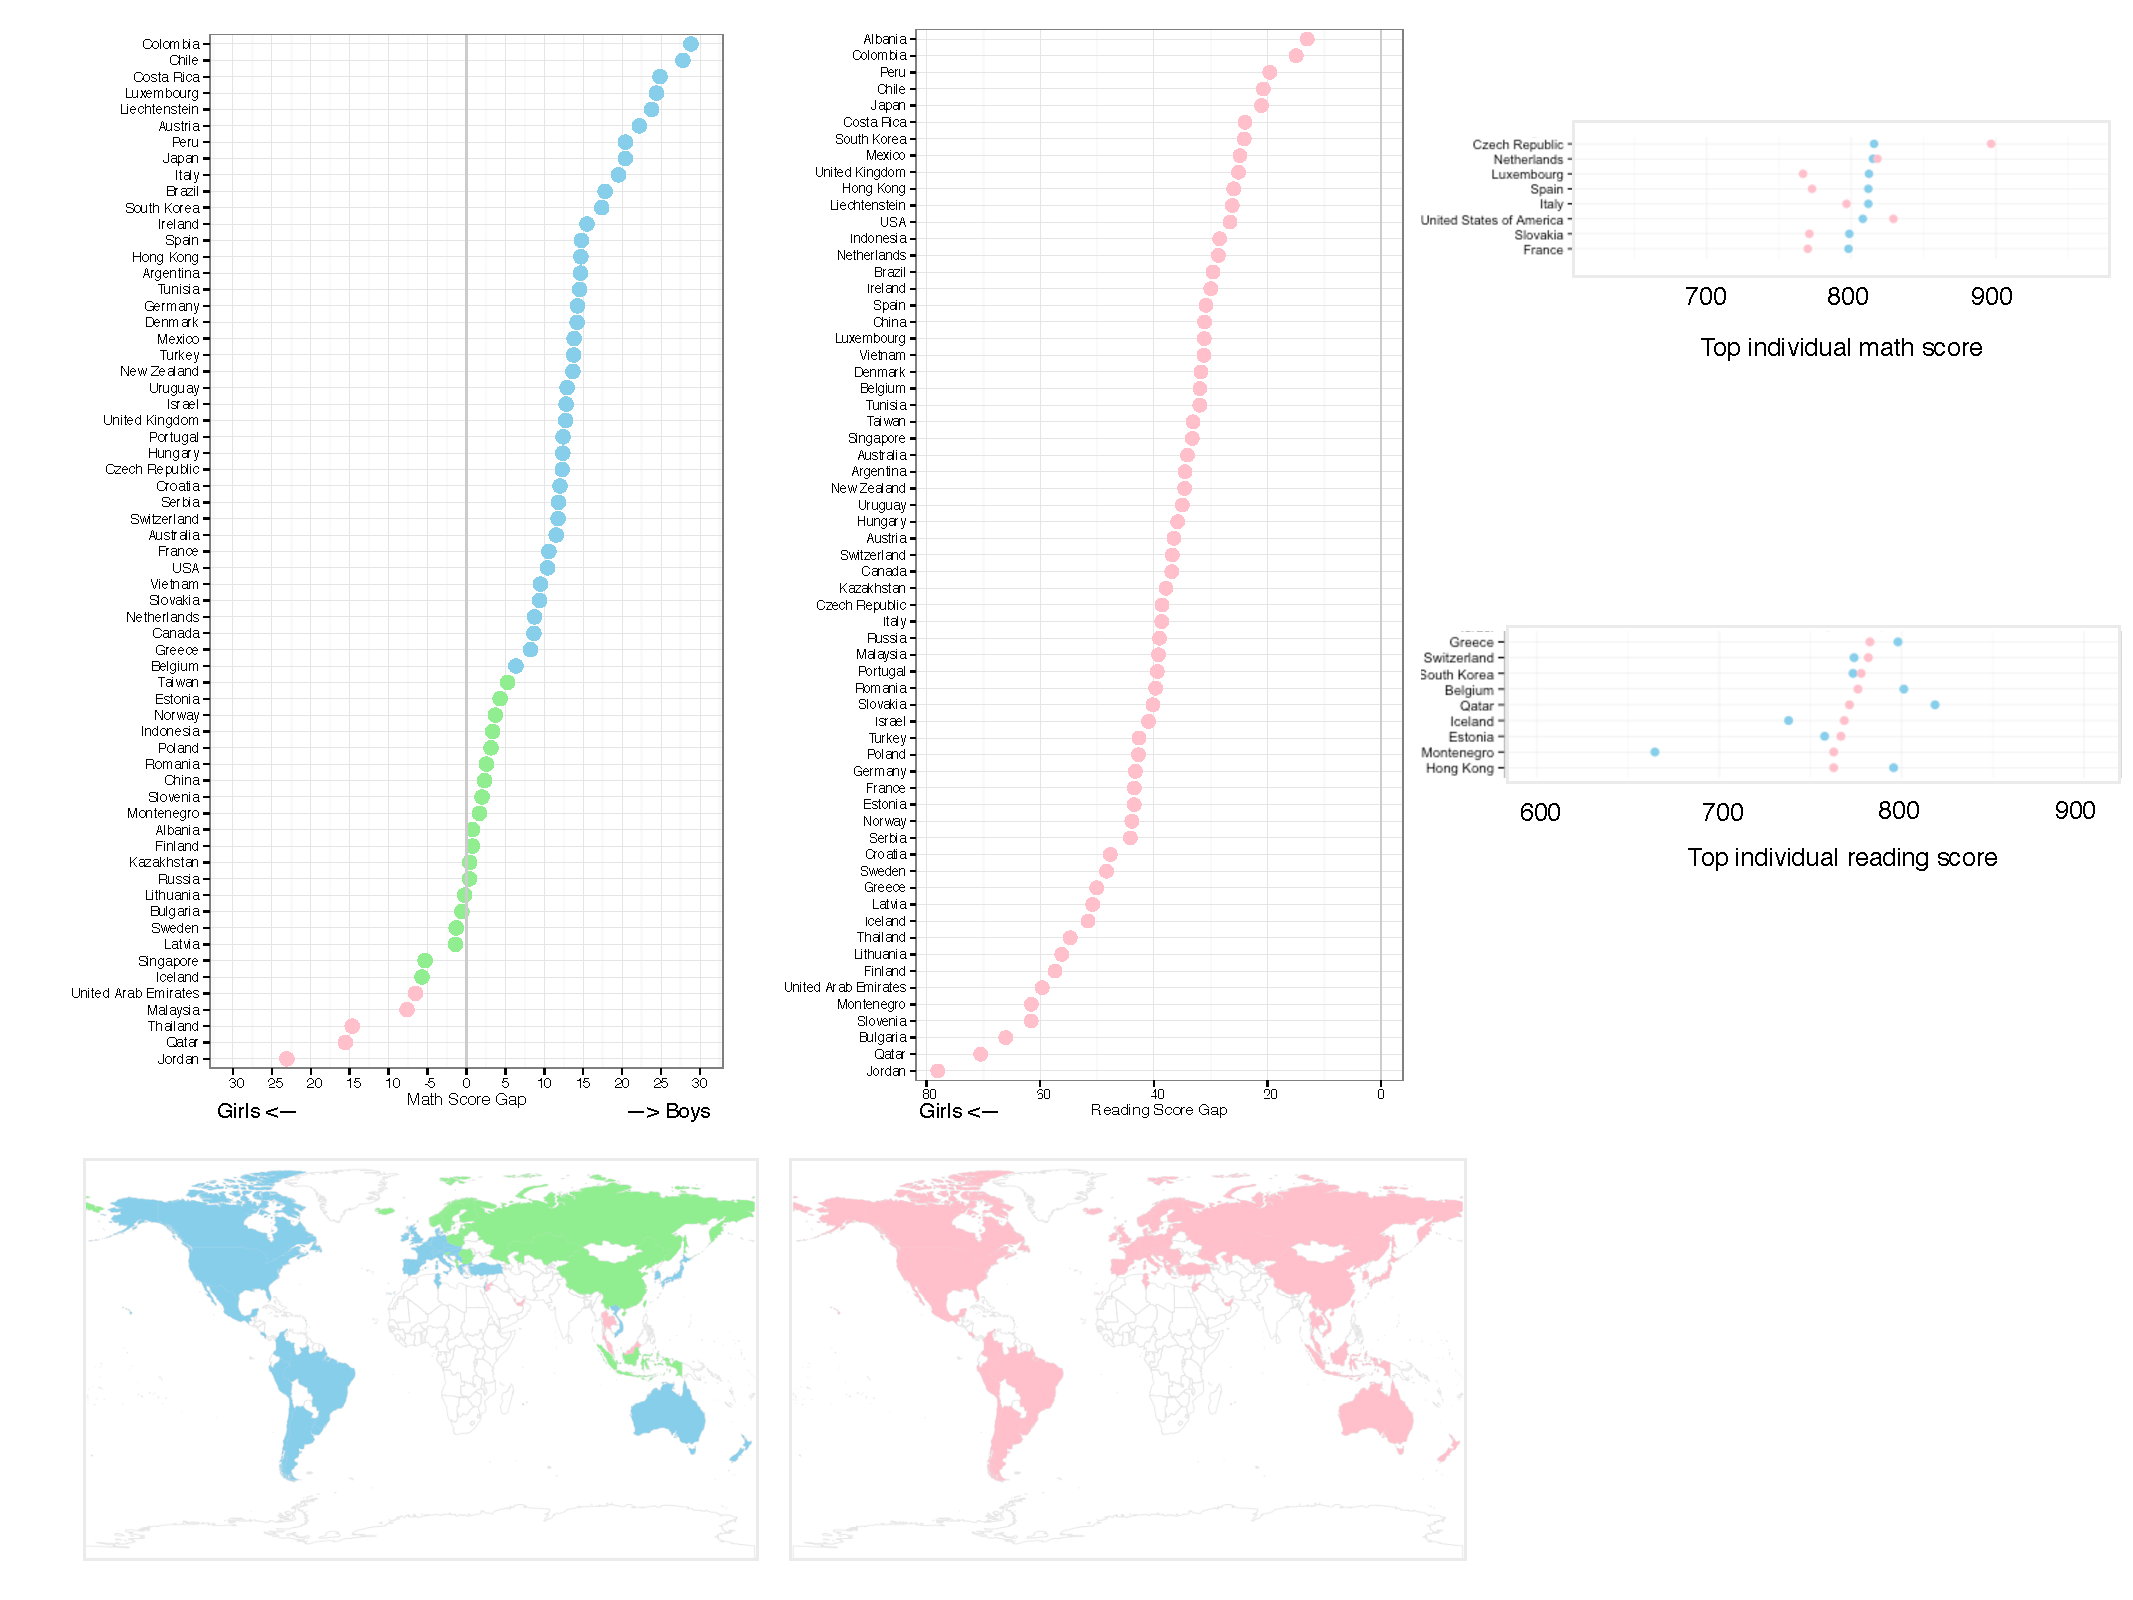
\includegraphics[width=0.95\textwidth]{images/PISA.pdf}}
\caption{Examining the gender gap in math and reading by country. Dotplots of mean difference shown by country, along with maps. Color roughly indicates magnitude of the gap, blue more than 5 points in favor of boys, green within 5 points, and pink more than 5 points in favor of girls. Surprisingly, this data indicates that the gender gap in math is not universal, many countries do not have a gaps, and a few countries show a gap in favor of girls. On the other hand, the reading gap is universally in favor of girls in all of the countries in this study. On an individual scale, the small plots show the top boys (blue) and girls (pink) score in a few countries, the story is different. Even in countries with a big gender gap in math, e.g. the USA has a 10 point gap, the top score for that year was attained by a girl. Similarly, for reading, individual boys top the reading score in many countries. One glaringly obvious deficiency in the data from the maps, is the lack of information from the continent of Africa.}
\label{OECD-gender}
\end{figure*}


\subsubsection{Elections}

\begin{figure*}[htp]
\centerline{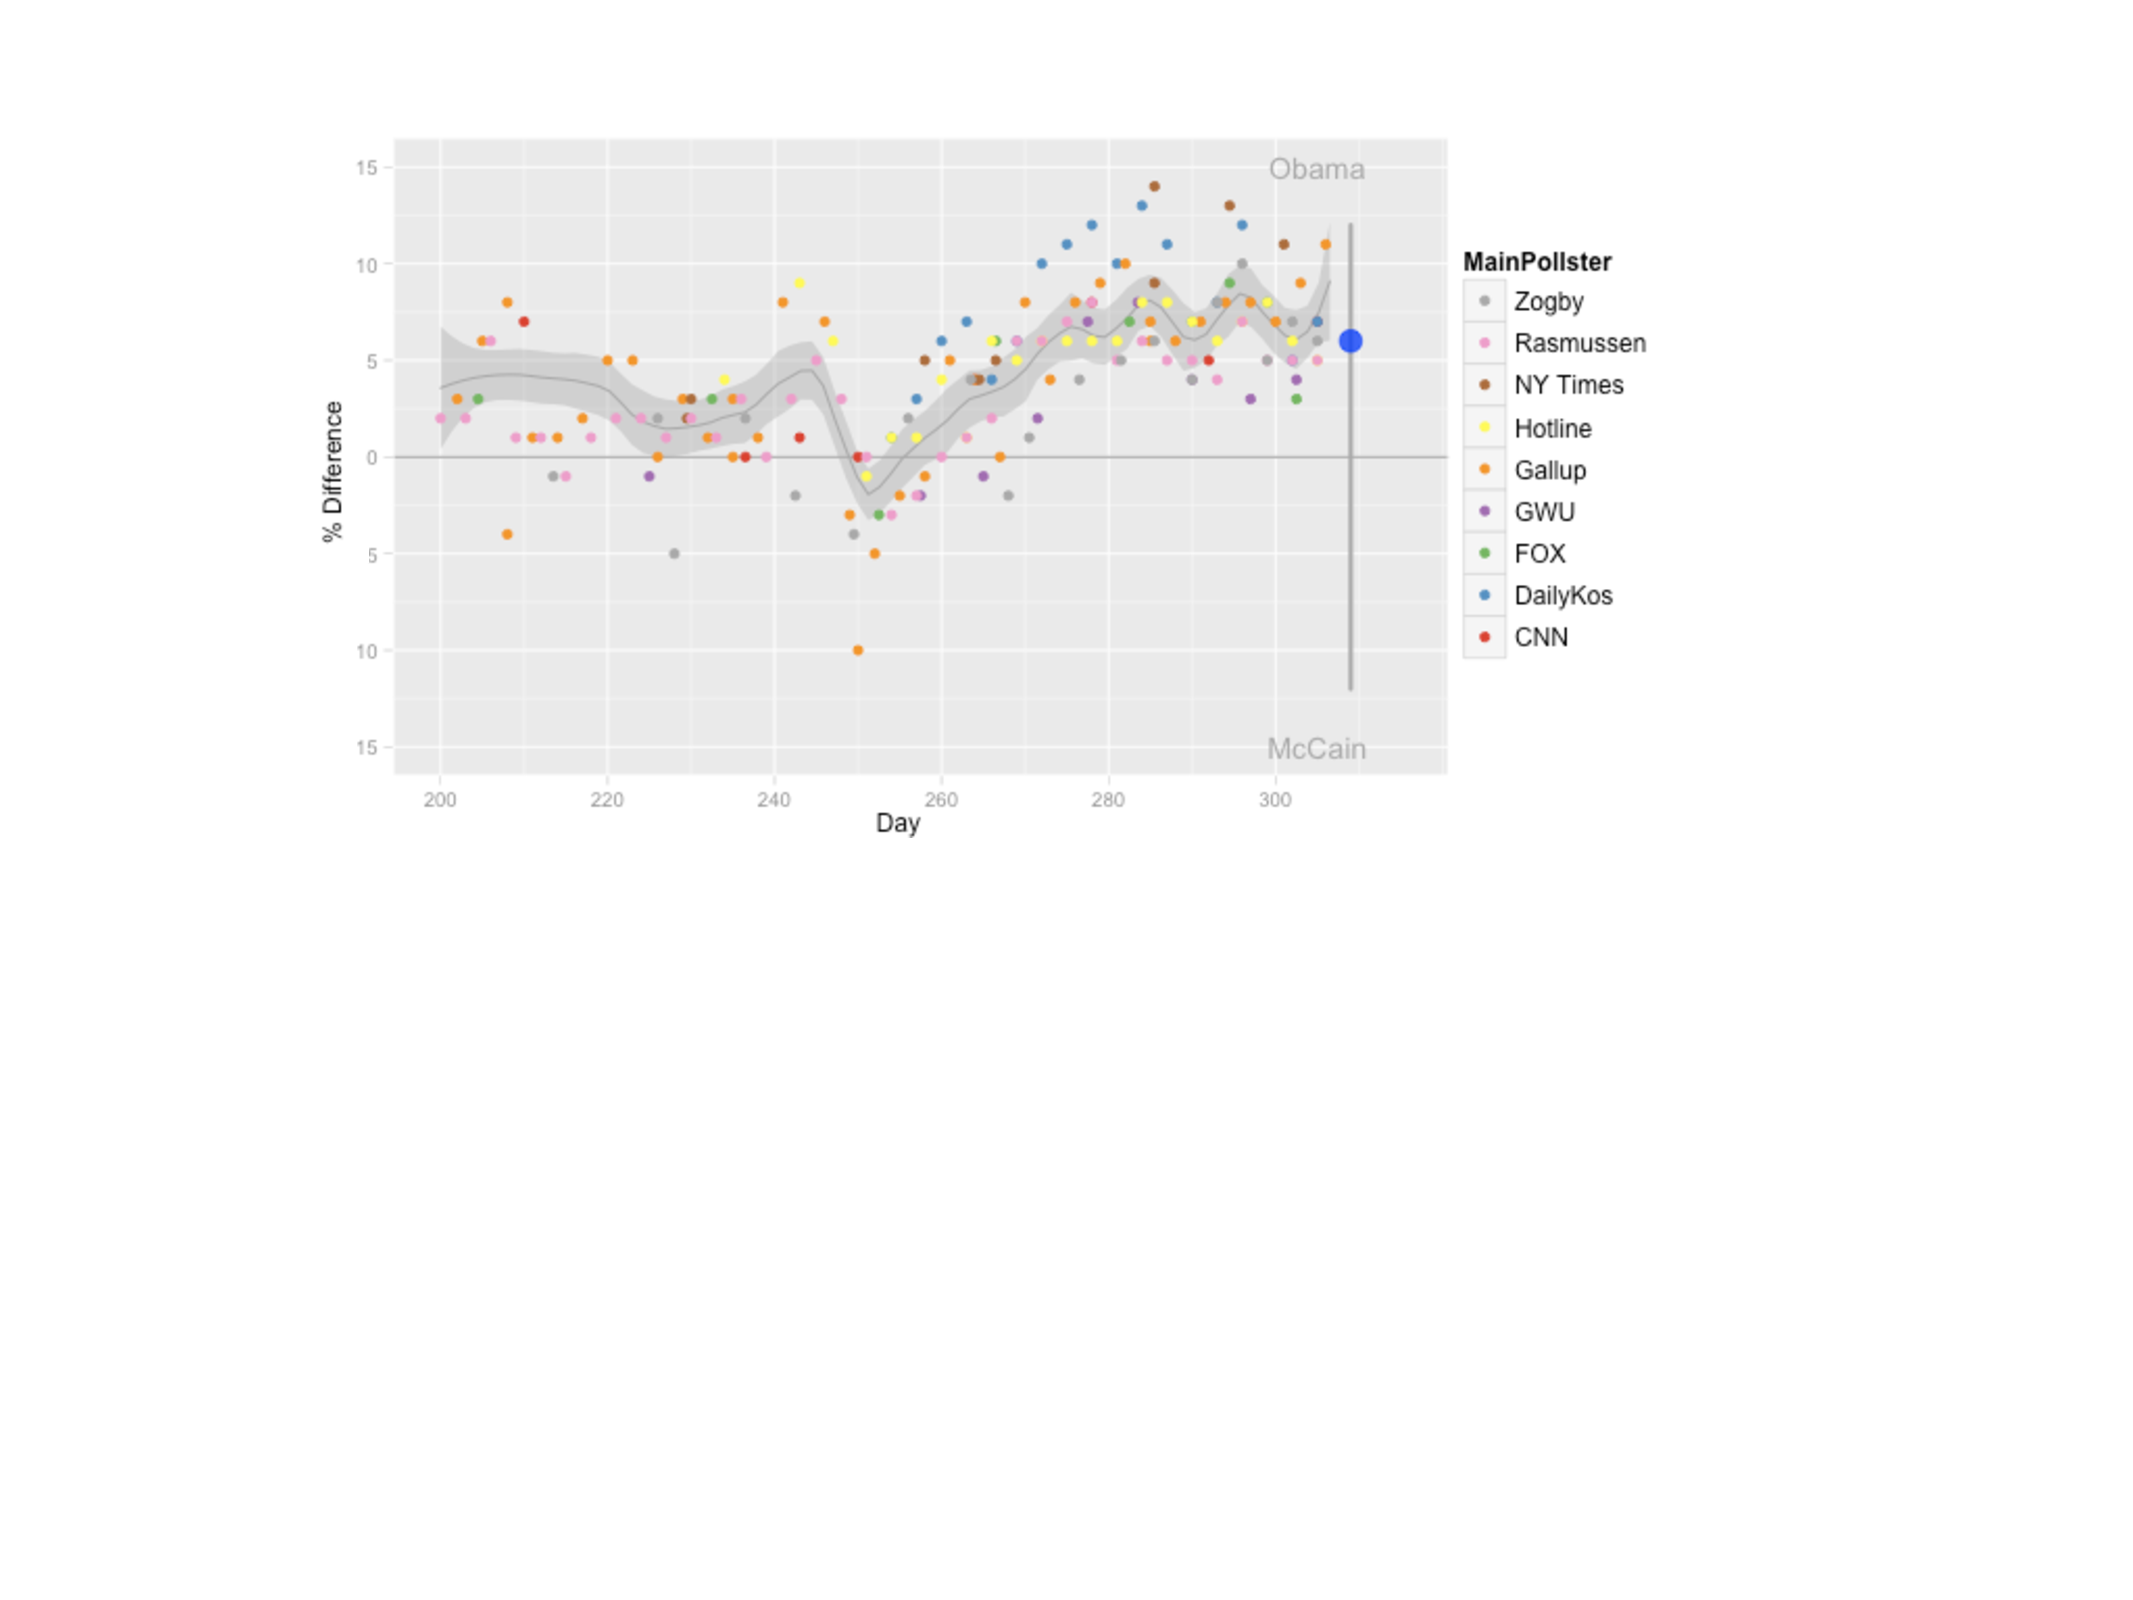
\includegraphics[width=0.95\textwidth]{images/elections.pdf}}
\caption{Tracking polls and final popular vote leading up to the 2008 US Presidential election. Percentage difference by time of poll release. Color represents pollster, gray strip shows poll average and the large blue dot indicates final election margin.}
\label{election}
\end{figure*}

In the 2008 US Presidential election cycle a young man called Nate Silver burst onto the world stage with an accurate prediction of an Obama win. His web site \url{http://fivethirtyeight.com/} (538) has expanded from politics to cover data stories in economics, science, life and sports. To obtain his accurate prediction of the election outcomes, he aggregated polls from different sources, but an important component was to adjust and weight the polls from different pollsters. Figure \ref{election} shows the polls from major pollsters, in the 100 days leading up to the election, as reported in \citet{mosley2010}. Percentage difference in percentage for Obama vs McCain is plotted against time the poll was released, as were made available on the web site \url{http://www.electoral-vote.com/}. Each dot represents one poll result, and color indicates pollster. The grey line and ribbon represents a loess smoothing \citep{CGS92} across all the poll results to indicate trend. There is a lot of variation in polls, even when conducted in very similar time frames. The variation in results can be as high as 10 percentage points.

Differences between polls produced by different pollsters can be seen. DailyKos light blue) is consistently higher than the trend, and consistently produced the most pro-Obama results. Rasmussen (pink) tended to be fairly close to the trend or below it (pro-McCain). Hotline (yellow) was varied early on in the season but closer to election day was near the average of all other polls. Gallup (orange) is noticeably varied, it has some of the most pro-McCain results as well as the most pro-Obama results. Gallup is a legacy American pollster who dates back to the early 1900s, and we would have expected that they would be providing more reliable polling numbers than observed. Interestingly the 538 web site now has detailed ratings of the major pollsters operating in the USA, and Gallup scores a poor C+. The plot of the national trend polls allows us to see the variability and the bias' of polling organizations. The pollster DailyKos, also known as Research 200, is a community action organization with political leanings towards to Democratic party. Actually it is one of the pollsters currently ``banned'' by 538! Rasmussen on the other hand has a reputation of leaning to the right, and currently has a large adjustment value to correct this on 538. Hotline is fairly neutral.

\begin{figure*}[t]
\begin{minipage}[h]{7in}
\centering
%\vspace*{.3in}~\\
$\vcenter{\hbox{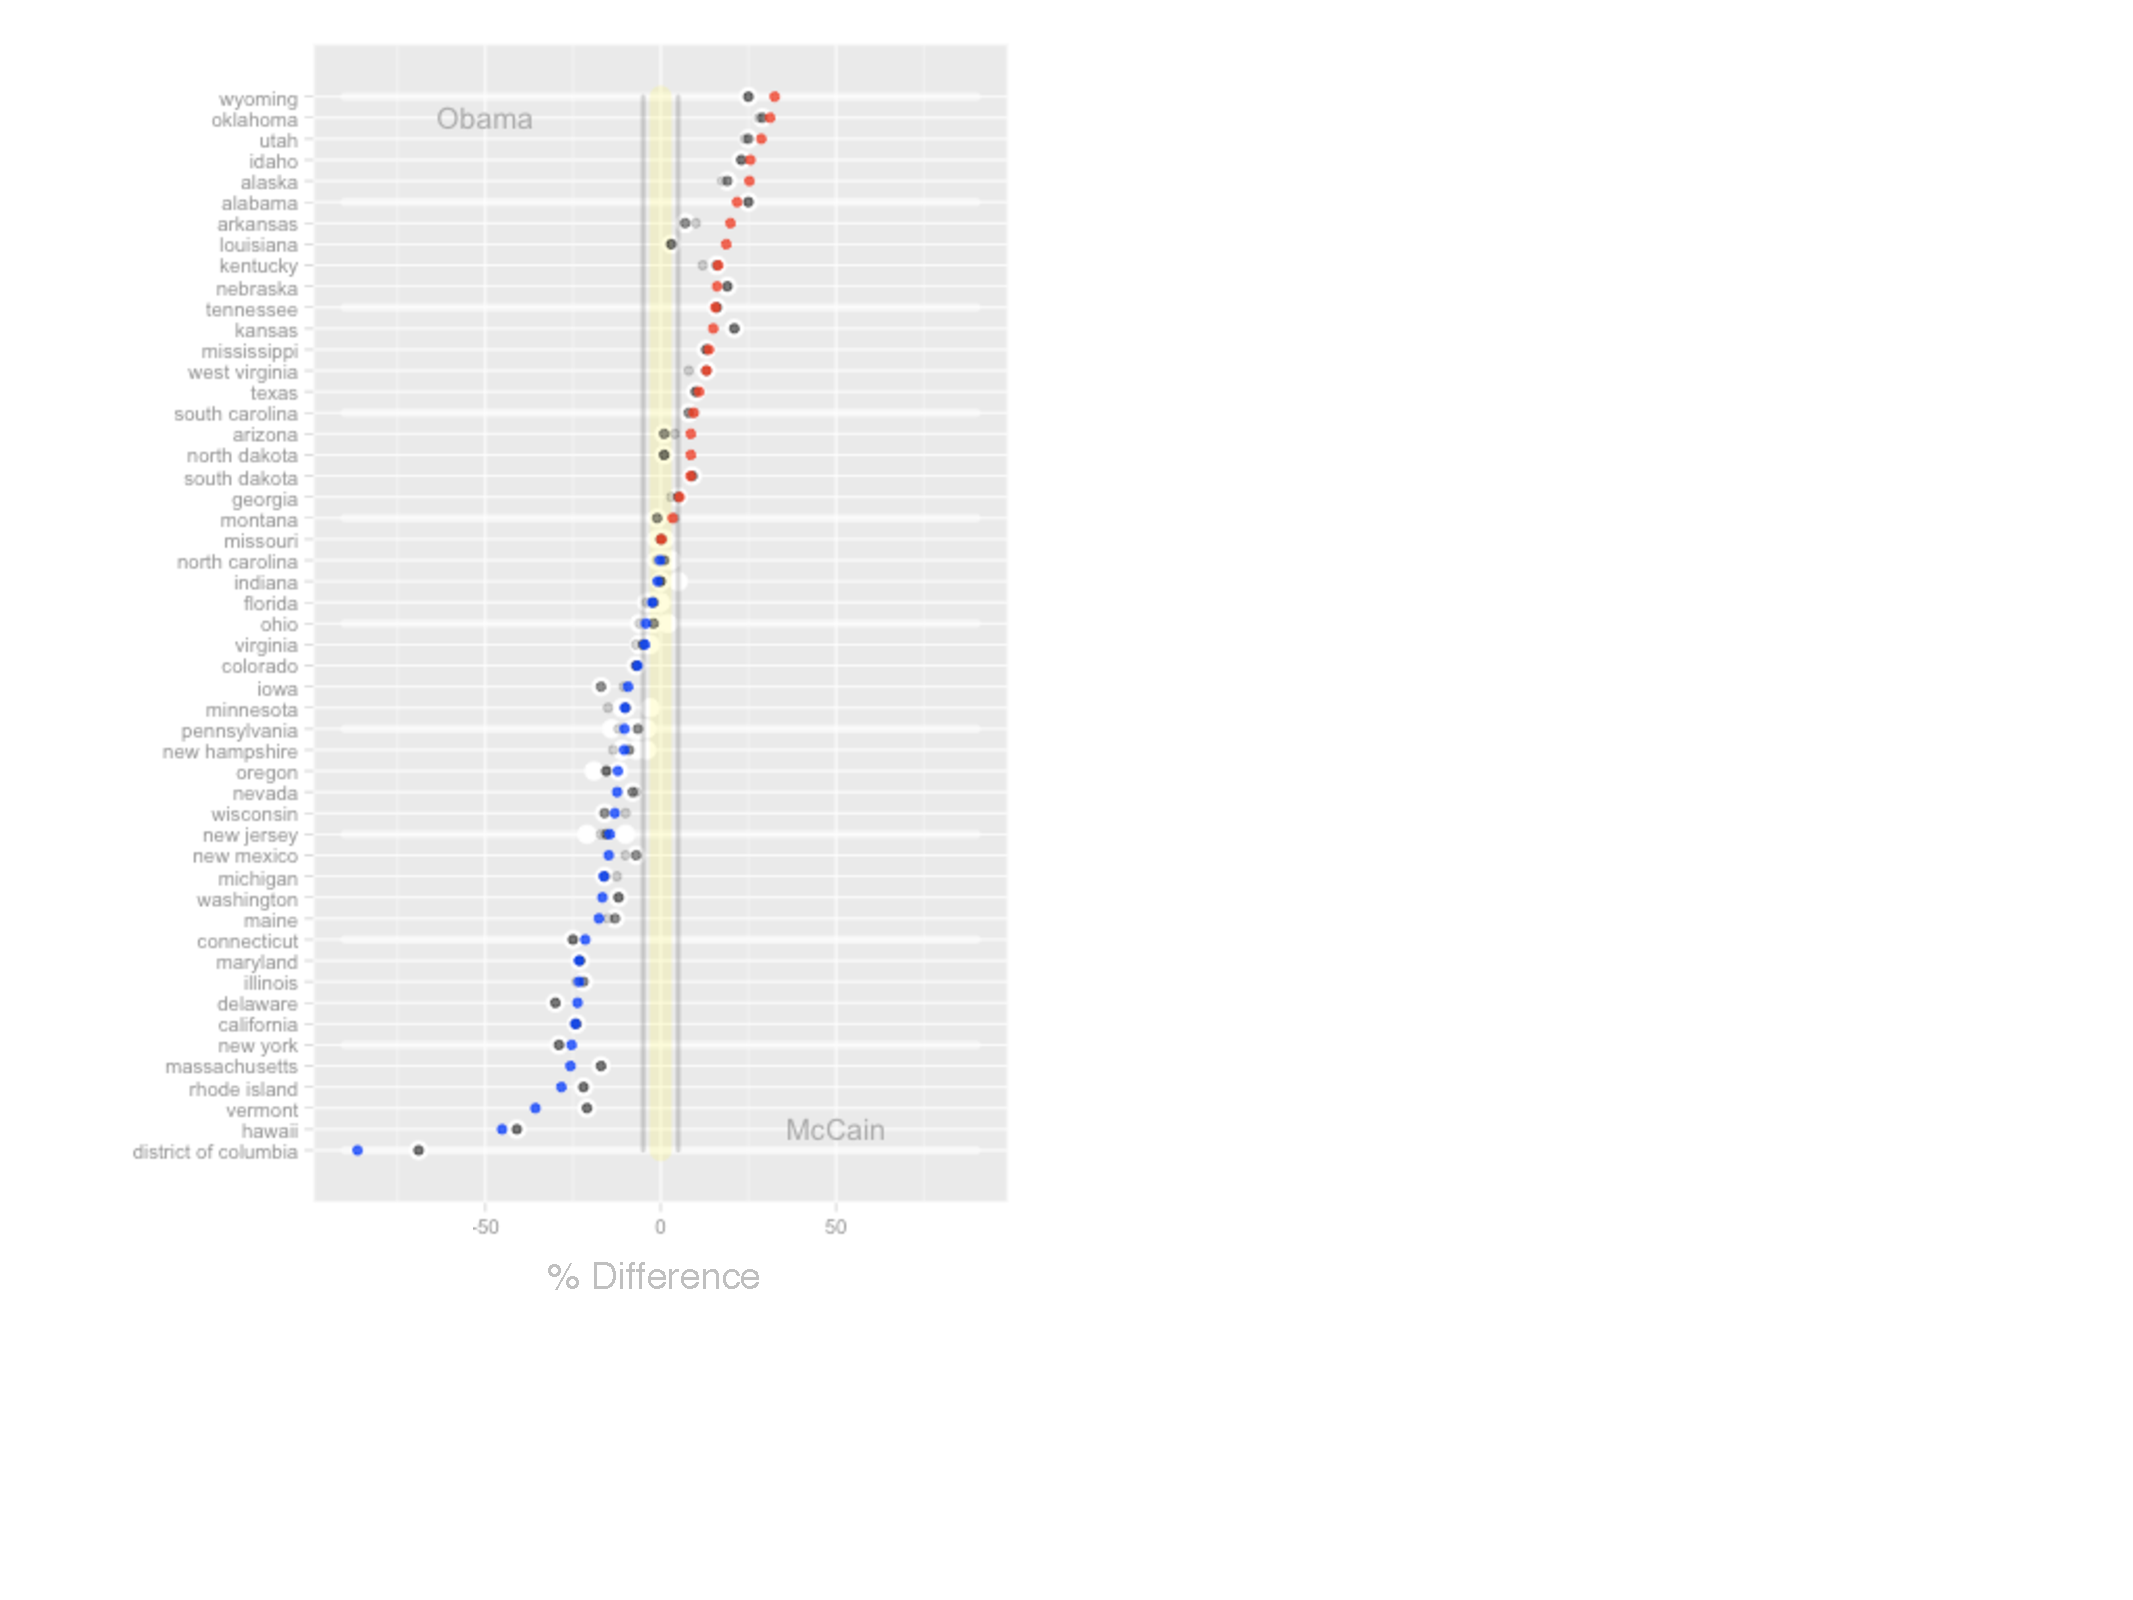
\includegraphics[height=4.5in]{images/elections2.pdf}}}$
\hspace*{.2in}
$\vcenter{\hbox{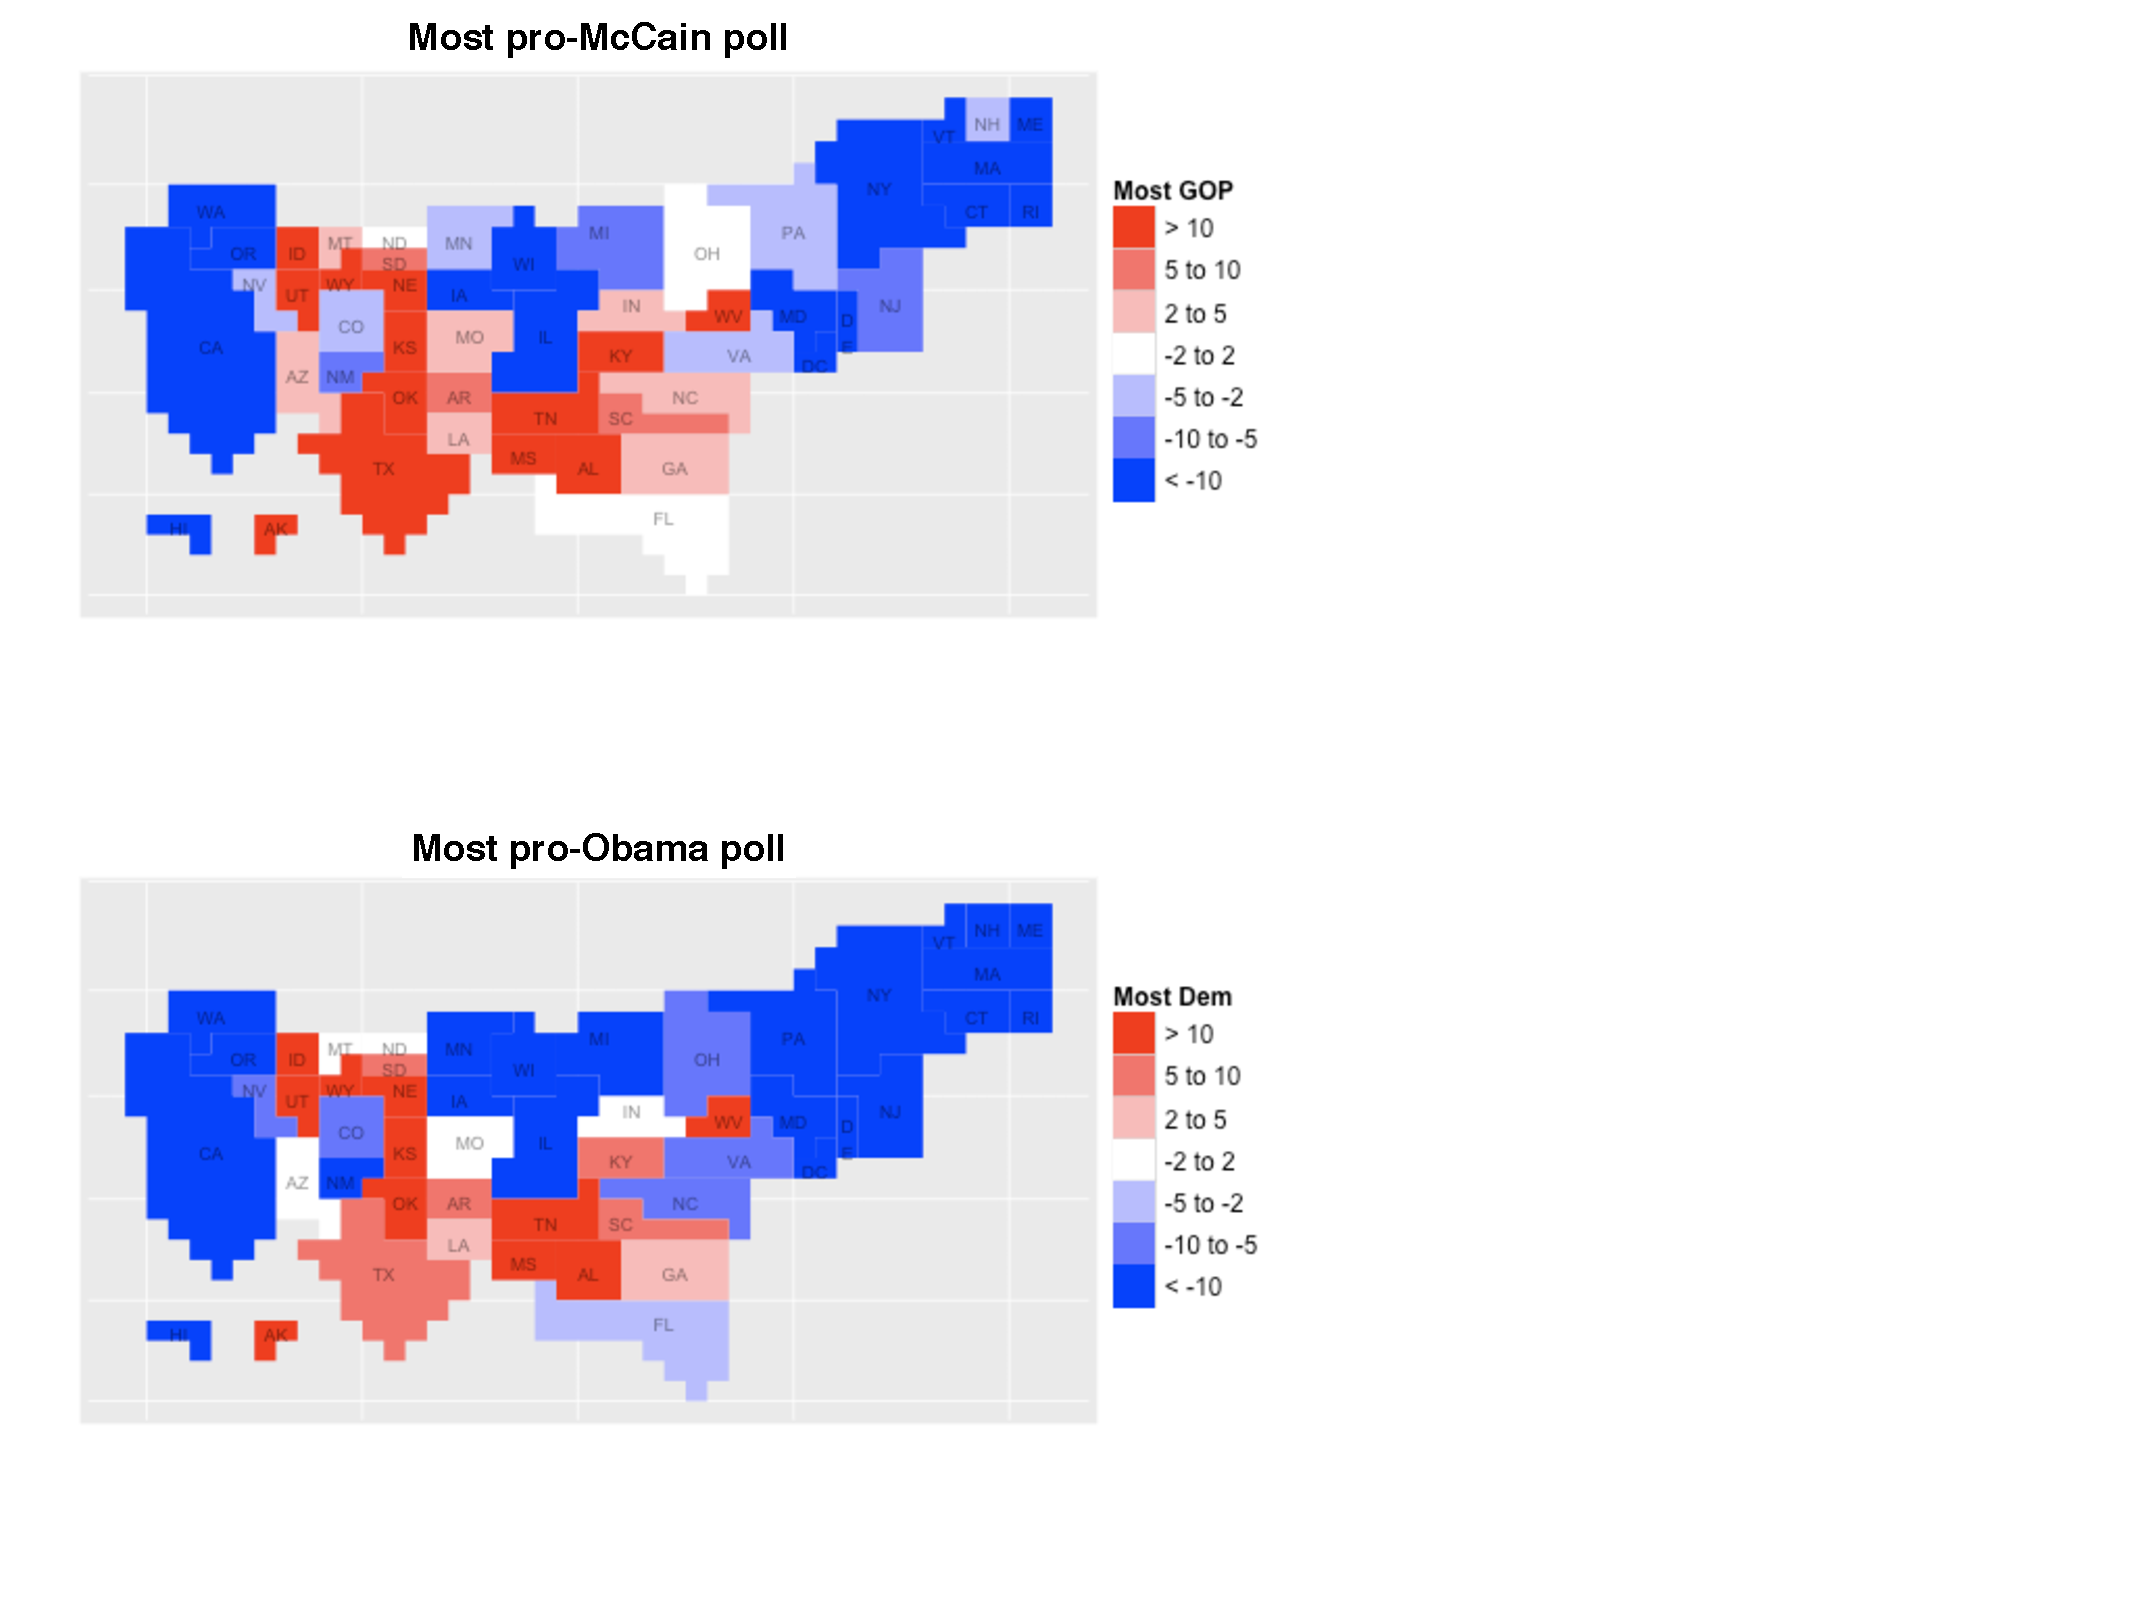
\includegraphics[height=3in]{images/elections3.pdf}}}$
\end{minipage}
\caption{Exploring variability in polls. (Left) Percentage difference by state, top to bottom ordered by McCain to Obama advantage. Color indicates final election result. Black is the median of all polls, grey is the median of the previous week's polls, and white shows all polls. (Right) Block cartograms, size of state represents electoral votes, colored by the most favorable poll result for each candidate, just prior to election day, in each state. In the best case scenario for McCain, the country still looks predominantly blue.}
\label{election2}
\end{figure*}

The US election is not won on the popular vote, though. Each state is assigned a number of electoral votes, roughly based on the size of the population. For example, in 2008 Iowa was worth 7 votes, whereas New York was worth 31. The electoral votes for most states as assigned based on winner take all: Obama won New York with 57\% in favor, so he earned all the 31 points. A candidate needs to tally up 270 or more points (of the possible 538, hence Nate Silver's web site name) to win the presidency. Figure \ref{election2} illustrates the state by state variation in polls. State, top to bottom most support for McCain to most support for Obama, is plotted against percentage difference. Each point indicates some result: the red/blue represents the final election result, black indicates the median of all polls, grey the median of the previous week's polls and white indicates all polls in that state. The yellow strip straddles a 5\% margin, with results in this range being states that are too close to call. States in these position tend to have a lot of pollsters operating, so there are more white dots visible, and for the most part it can be seen that the final result closely matched the poll results. There are a couple of exceptions: Montana was predicting to be a toss-up but ended up being more for McCain than expected, and Iowa ended up closer than the latest polls predicted. During the election cycle, we produced these plots and animated them from the previous week, which allowed obtaining a sense of temporal shifts in attitude, and the variability leading up to the actual vote.

In the 2012 season, this work was expanded to explore the effect of political action committee spending, after the 2010 Supreme Court decision enabled unlimited election spending by organizations \citep{kaplan2012}. And the 538 site is expanded to an independent news site and is an exemplary location to browse to read examples of numerically and visually analyzing large data du jour.

\subsubsection{Airline Traffic}

Every few years, the graphics and computing sections of the American Statistical Association provides a data challenge, the Data Expo (\url{http://stat-computing.org/dataexpo/}), and encourages students, faculty, industry statisticians to make a visual analysis. In 2009 the data consisted {\em ``of flight arrival and departure details for all commercial flights within the USA, from October 1987 to April 2008. This is a large dataset: there are nearly 120 million records in total, and takes up 1.6 gigabytes of space compressed and 12 gigabytes when uncompressed.''}.

There were 9 entries, four of which won prizes, and are described in short articles. \citet{expo-wicklin} used SAS to produce a number of informative displays about departure delays air travel in the USA: calendar view summaries show differences between years, months and days of the week, time series display volume of traffic and weekly cycles, and a heatmap is used to compare carriers over the time period. This was a lot of data displayed very succinctly, providing key details of flight delays. \citet{expo-wickham} tackled a smaller task, comparing operations at two different airports, and \citet{expo-dey} focused on a model to find the path of least delay between any pair of airports.

\citet{expo-hofmann} explored many aspects of the data. Maps of origin to destination show which carriers operate on a hub system and which don't. Time series of volume at major airports show effects of events like the 9/11 tragedy. Side-by-side boxplots were utilized to display delays by airport, revealing the problematic EWR, SFO, ORD, LGA and the efficient operations of DTW, MSP and DFW (Figure \ref{airlines2}). Facetted scatterplots with overlaid loess fits show trends in delays by carrier. This group also looked for ``gaps'' in the data, where planes are last seen at one airport, and then magically appear at another airport. These gaps correspond to ghost flights, planes that fly passengerless, in order to get a vehicle into a location that it is needed. It represents inefficiency in operations. Most carriers have been reducing this costly operation, but Northwest airlines had an increase in the latter few years of this data. Delta, which merged with Northwest in 2008, saw improvement in efficiency. Interactive graphics was employed to examine different chunks of the data, like the relationship between fuel consumption, distance flown by carrier and year (Figure \ref{carrier-efficiency}). Basic plots revealed that many problems with the data, flights leaving 12 hours before they were scheduled (Figure \ref{airlines1}), several hot air balloons that travel 430 miles per hour, and more than 200,000 flights of less than 50 miles. Stringing delays together with weather patterns revealed the problems that strong cross-winds cause at airports. And using some interpolation between geographic locations of airports, the departure and arrival times, allowed animating air traffic flow across the nation (\url{https://vimeo.com/119233995}).

\begin{figure*}[htp]
\centerline{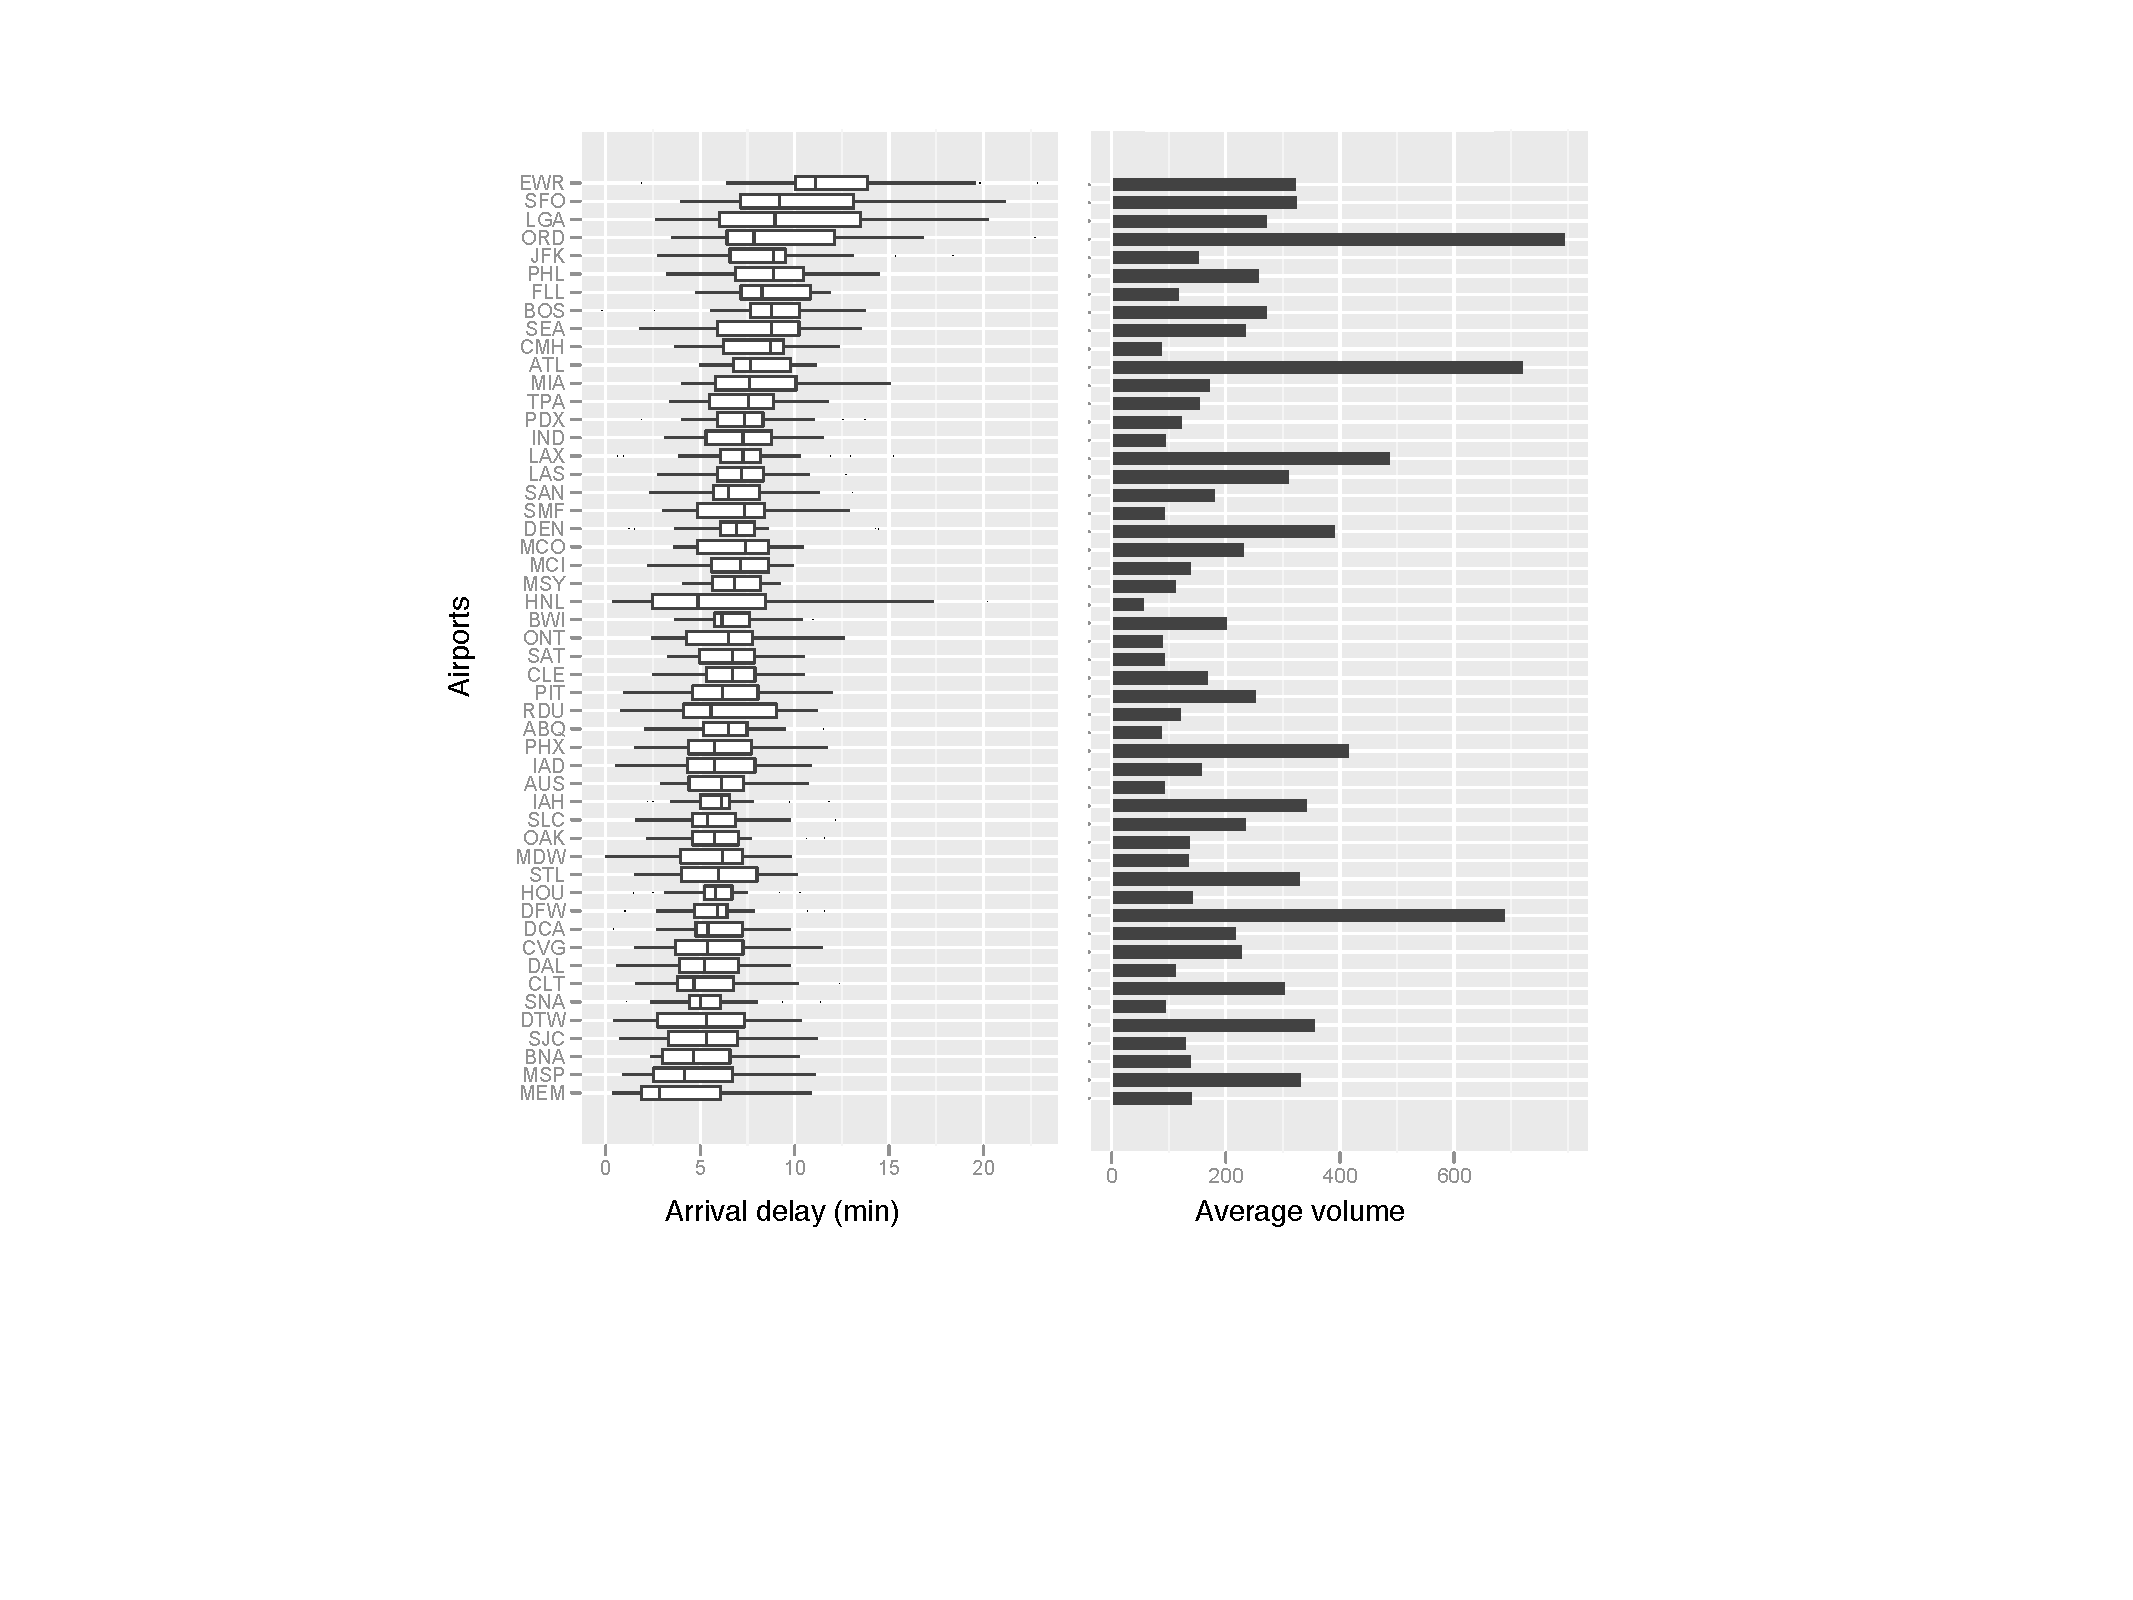
\includegraphics[width=5in]{images/airlines2.pdf}}
\caption{Arrival delays by airport, sorted top to bottom from worst average delay to least, and volume of traffic. Only the top 50 airports based on delay are shown. Over this time period EWR (Newark, NJ) had the worst record in delays even though their traffic volume was not large compared to other airports. ORD (Chicago, IL) had a bad delay record, but they also have the highest volume. DFW (Dallas-Fort Worth, TX) compared favorably with low average delays and very high volume.}
\label{airlines2}
\end{figure*}

\begin{figure*}[p]
\centerline{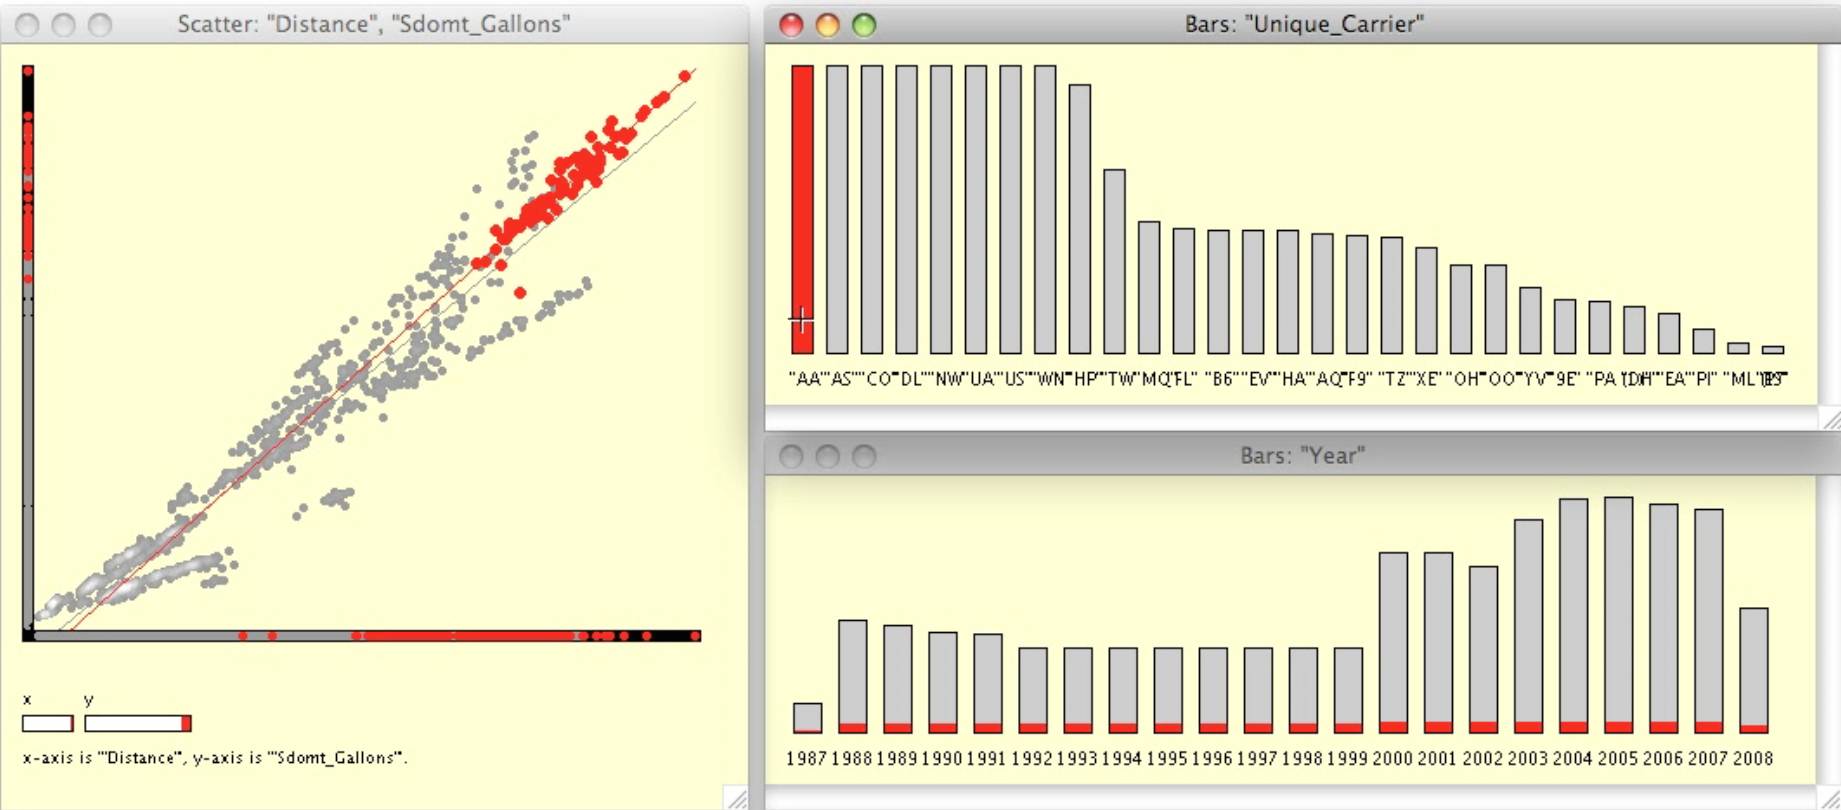
\includegraphics[width=5in]{images/airline-manet1.png}}
\smallskip
\centerline{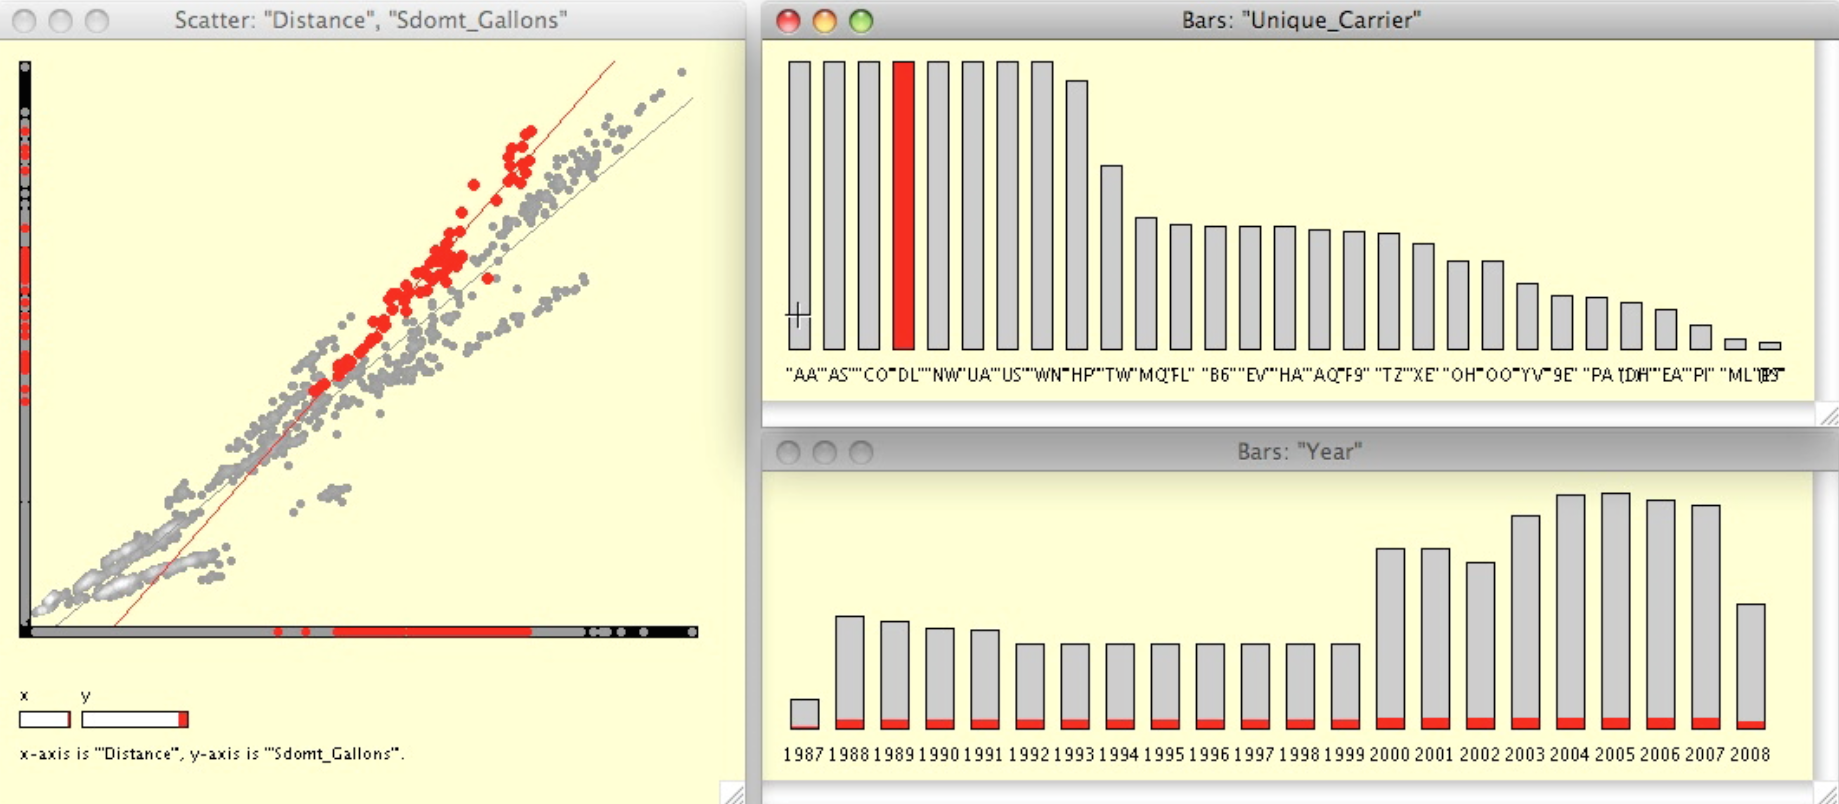
\includegraphics[width=5in]{images/airline-manet2.png}}
\smallskip
\centerline{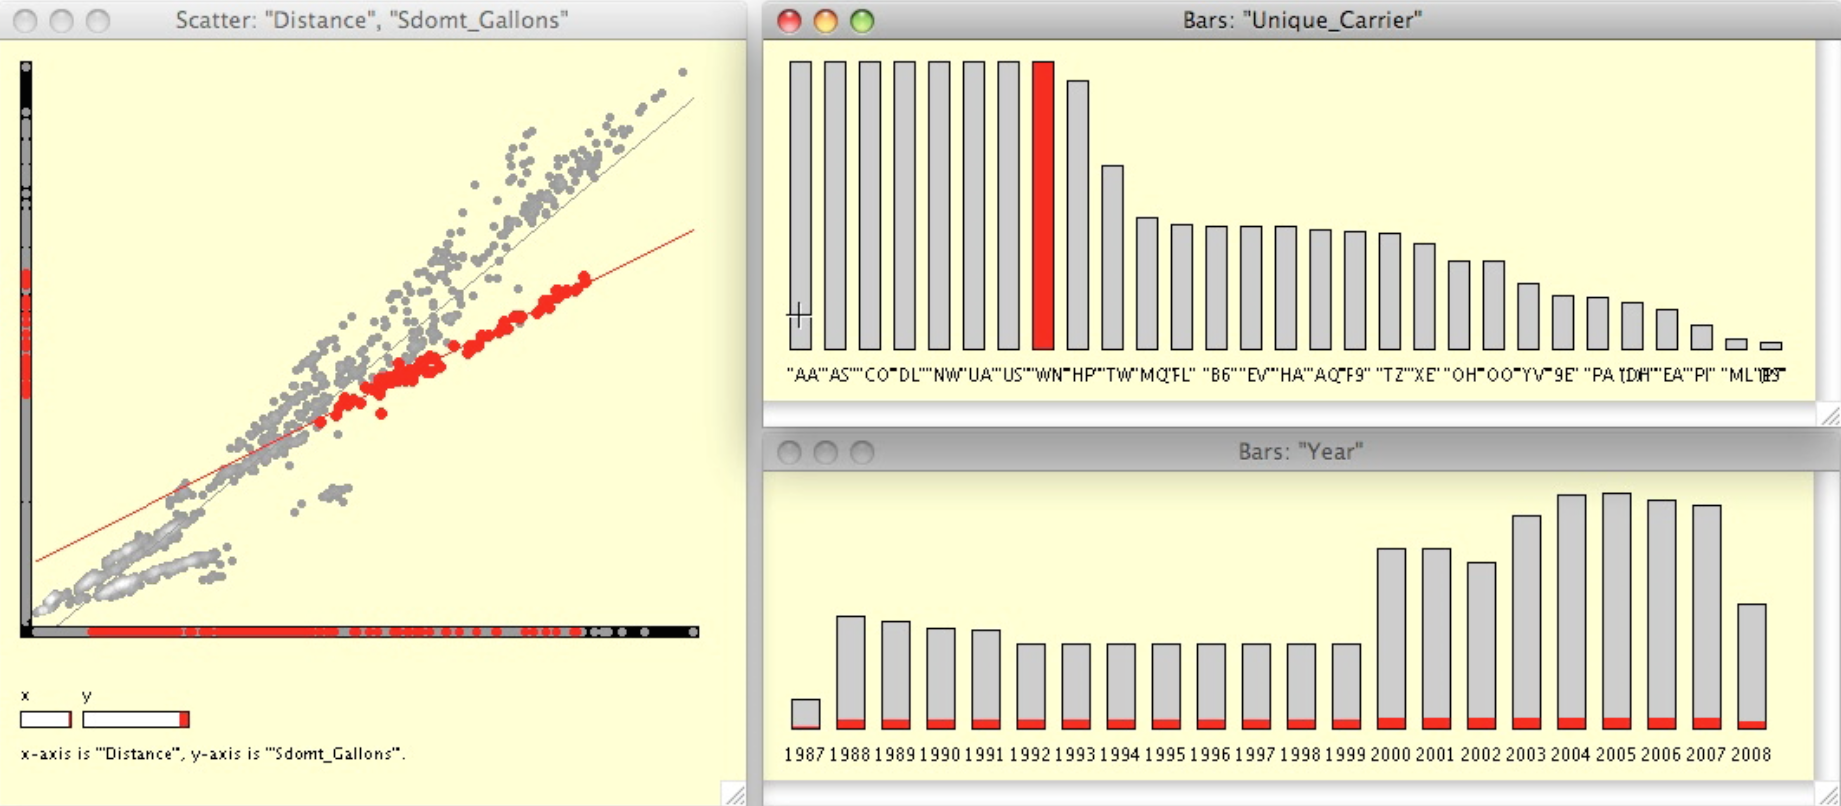
\includegraphics[width=5in]{images/airline-manet3.png}}
\caption{Three snapshots of interactive graphics using the software MANET on a processed chunk of data to explore carrier efficiency. Fuel consumption (vertical) is plotted against distance flown (horizontal) in the scatterplot, and bar charts show carrier, and year. Three airlines are highlighted (red) from top to bottom: American Airlines (AA), Delta (DL) and Southwest (WN). American Airlines is at the top of the pack: big carrier, big consumer. Over this period of time, Delta is relatively inefficient, having relatively higher fuel consumption for the same distance flown. In recent years, which can't be seen in this data, they have improved substantially. Southwest is a big carrier but has substantially more efficient fuel consumption than their competitors.}
\label{carrier-efficiency}
\end{figure*}

\begin{figure*}[t]
\centerline{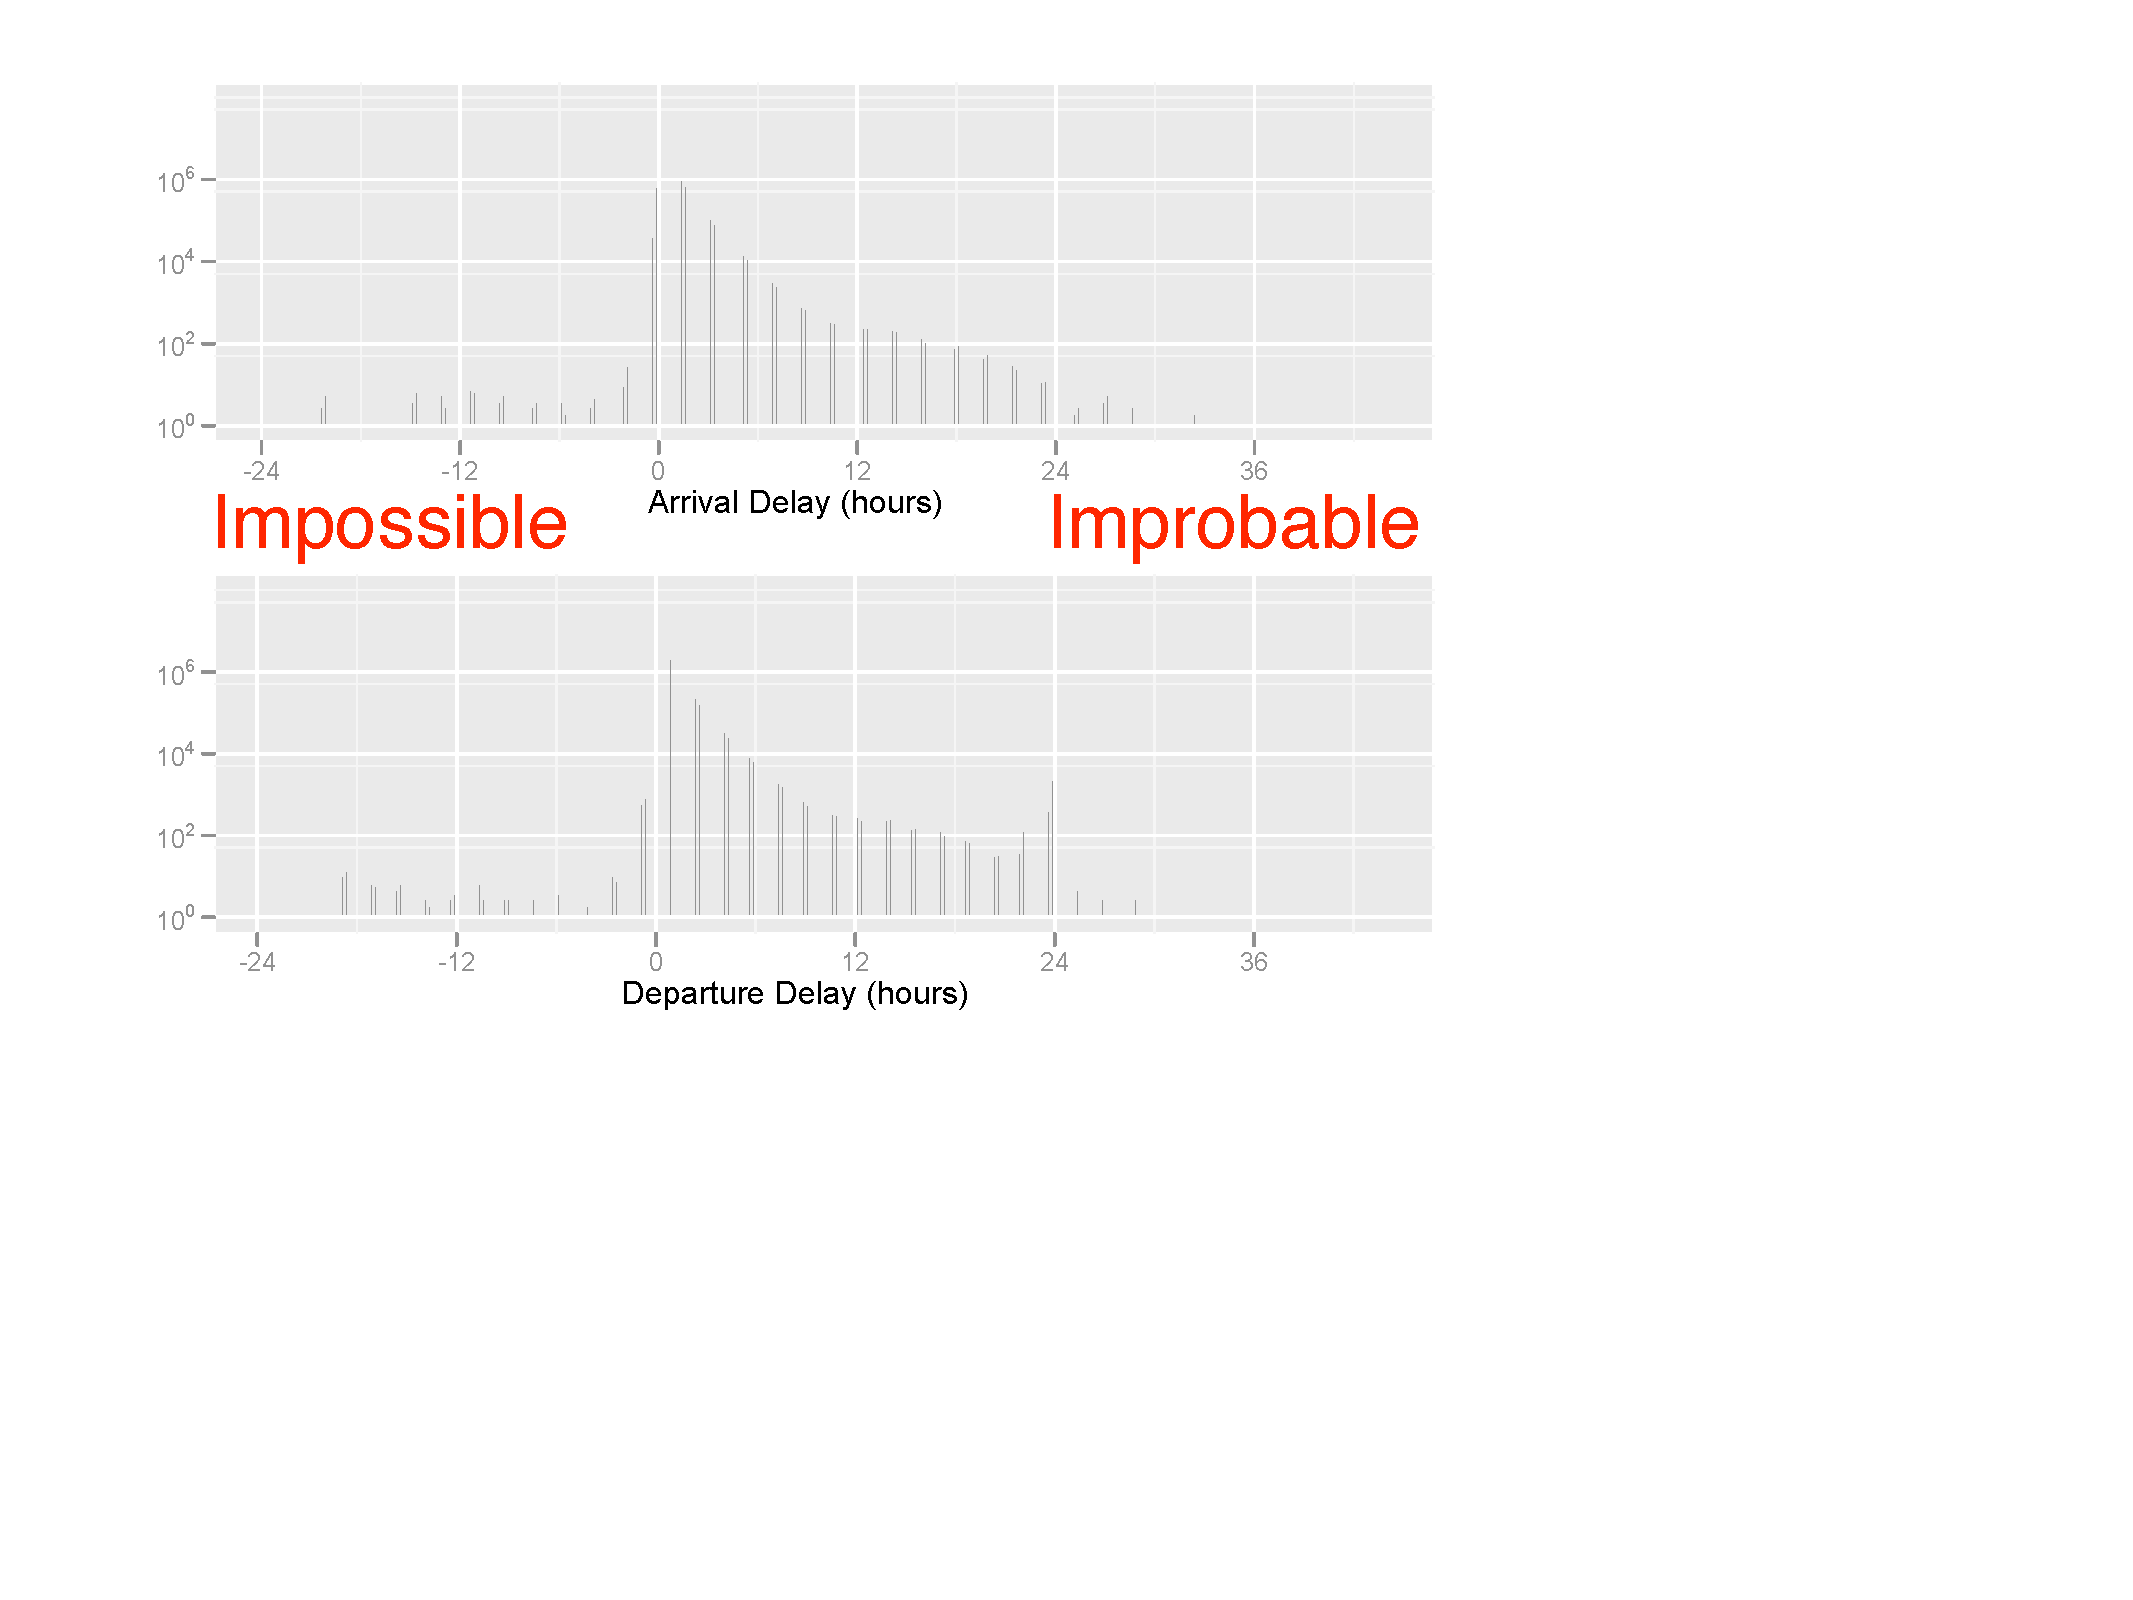
\includegraphics[width=5in]{images/airlines1.pdf}}
\caption{Histograms showing arrival and departure delays across carriers, airports and years. Delays aggregated in 15 minute bin widths. Arrival delay is calculated from the difference between the reported actual and scheduled departures. Arrival delays of -24 hours would be a plane that left a day early, which we would expect is impossible. }
\label{airlines1}
\end{figure*}

\subsubsection{Wikipedia}

Wikipedia (\url{https://www.wikipedia.org/}) is a collaboratively written encyclopedia, that is a huge resource for the general public. Because it is a primary example of mass editing, the flow of edits is potentially interesting. This problem was tackled by \citet{wiki}, with an associated web site \url{http://fernandaviegas.com/wikipedia.html} where you can see some of the visualizations. The book chapter describes the process of pulling the data, pre-processing and making visualizations of different aspects. Their endeavor began in 2003, early days for the encyclopedia. As an example of the magnitude of the data, the page on ``Microsoft'' had 198 edits generating 6.3 megabytes of text, and the page on ``Cat'' had just 54 edits.

The edits data is huge. To tackle is Wattenberg and Viega, initially created an interactive visualization for single pages. They use a modified parallel coordinate plot \citep{In85,We90}, which might also be considered to be a variation of a hammock plot \citep{hammock,ggparallel}, with versions as the variables, and text size as the stripe thickness. Stripes are colored by author, so individual contributions to pages can be tracked. (Anonymous editors are grey.) The overall height of the plot indicates the length of the article. There are two prominent examples shown: ``chocolate'' and ``abortion''. The displays enable some information to be immediate: if there is ownership of a page by a few editors then there are a few differently colored stripes. The page for ``abortion'' has a big empty patch indicating tha the entire page was erased temporarily, probably by a malicious editor. Tug-or-wars between editors can be seen in some politically or emotionally controversial subjects. Interaction is provided to trace editors contributions and to see the actual text that was edited.

With big data, we see that there are many different choices in what to plot. Here, the authors chose to tackle the problem using the page as a basic unit. In a secondary task their basic unit is an editor, and a new display called a chromogram {\color[rgb]{0,0,1} \citep{wattenberg2007visualizing}} is employed to enable viewing how an editor has contributed to wikipedia.  These both would be considered to be drill downs into the data, because each shows a very narrow slice of the data. There are now 4,714,447 pages, to visit each one would take some time. Ideally, approaching a problem as large as this would also provide some larger visual overviews: number of pages over time, number of authors over time, how many pages different authors edit, ... and provide some comparative views, pairs of pages for example, or hierarchical topic lists, or how pages link to each other. The data implores the analyst to display it in many more different ways. The web site \url{http://infodisiac.com/Wikimedia/Visualizations/} illustrates ways that many other people have tackled visualizing wikipedia.

Raw information in the form of text provides new challenges for visualization. Universally, people have adopted the use of tag clouds to display word frequency of blocks of text, e.g. wordle \citep{wordle}. But there is more to understanding patterns of text than showing frequency. Some good examples of processing text data and visualizing different facets of text can be found in \citet{jockers} who examines British literary history. New tools for grouping text into topic models using latent dirichlet allocation have been developed, and the R \citep{R} package LDAvis \citep{LDAvis} provides ways to interactively visualize the data.

\subsubsection{The San Francisco Housing Crisis}

Another book in the Beautiful series is ``Beautiful Data'' and in that volume you will find an article by \citet{SFHousing} that illustrates visually exploring the housing crisis with an early version of the R software ggplot2 \citep{wickham2009ggplot2}. This package is now almost ubiquitously used for plotting data. This book chapter is is an extraordinary example of pulling data from the web, cleaning and displaying it in different ways to learn about events that affect our lives. The explanation of the process is superb.

The story of the housing crisis begins by studying the temporal scale: average prices and number of sales from 2003-2009. We can see the average house price double over this period, and then drop by half starting summer 2007. Sales tend to cycle some, showing some seasonality, but clear decline starting in 2006. Interestingly, sales tick up again early in 2008 after sharp declines in average price. The authors then examine economic conditions, and compare inflation adjusted,  alongside unadjusted, average price to learn that these two measures started diverging mid-2005. The two had not converged by 2009.

Breaking the data into house price deciles, and examining these relative to the median house value shows that the disparity in house prices is expanding, supporting a perspective that the more expensive houses are becoming relatively more expensive. Drilling down into each geographic regions shows that there are some areas of the city that are more affected than others: San Pablo experienced the full brunt of the boom and bust but Berkeley saw barely a hint of decline. Plotting  geographically  reveals that the eastern part of the city experienced more turnover in houses. Comparing price decline and demographic factors revealed that higher income areas, and higher percentage of college grads saw less decline, while areas where residents had longer commutes saw bigger hose price declines.

This article illustrates elegantly how visualization can be used to explore data.

\subsubsection{Credit card purchases}

\citet{hand2000} is an early article explaining data mining, using a large Barclay's credit card transactions database as the example. The reason to read this article is see how the humble histogram can be priceless for exploring big data. The histogram, with carefully crafted $\pounds$1 binwidth, is used to display petrol (gas) purchases, and department store spending. We might expect that in department stores there to be strong peaks just before the whole pound, and it is exactly what we see. But to see similar patterns in petrol purchases is a surprise. There are large peaks in petrol purchases at $\pounds$10, $\pounds$15 and $\pounds$20, and to a lesser extent $\pounds$12, $\pounds$25, and $\pounds$30. This behavior is driven by the consumer rather than the price points of store products -- clearly some drivers, a lot of drivers, like to spend whole nice round whole pound amounts when purchasing petrol. Beyond these peaks, the distribution looks close to bell-shaped, centered at $\pounds$20.

Working with huge amounts of data can often be done with basic statistical graphics. There are a few cautions. Bars of small counts get lost easily with big data, which might result in failing to observe rare events. Basic scatterplots may suffer from overplotting.  Scaling up of basic statistical graphics does require some care.

\section{Review of the Literature}


There is a scarcity of papers on visualization of large data in the most likely statistical journals, e.g. Journal of Computational and Graphics Statistics, Computational Statistics, Annals of Applied Statistics. Papers that do focus on graphics are fairly associated with small data, an special statistics-related purposes, rather than providing solutions to visualizing large amounts of data. The most reliable source is IEEE Transactions on Visualization and Computer Graphics. The papers presented at the annual InfoVis conference are published in this journal in one of the last two issues of each year. A less formal, but very visible resource, the CRAN archive (\url{http://www.r-project.org/CRAN}) contains several recently contributed packages that are useful for working with large amounts of data.

\begin{itemize}
\item Scatterplots

One of the most useful methods for viewing multivariate data, the scatterplot matrix \citep{scatmat}, is less useful when there are more than a handful of variables. Even plotting pairs of variables separately, putting them in a loop to animate the display of all pairs is infeasible when the number of variables is really large.  \citet{wilkinson2005graph} resurrected Tukey's ideas on scagnostics \citep{TukeyTukey1985}, to provide automated ways to extract pairs of variables that might be the most interesting to plot. Their approach is to calculate nine measures for interesting features in the scatter plot - outlying, skewed, clumpy, sparse, striated, convex, skinny, stringy, and monotonic - based on proximity in graphs. The methods are implemented in an R package \citet{wilkinson2014package}, and a standalone software, ScagExplorer \citep{dang2014scagexplorer}.

When the number of cases is large, but the number of variables is small, reading distributions from scatterplot can be nebulous because points will be overplotted. \citet{carr-scatmat} approached this with a modification employing density plots, for which the recent {\tt hexbin} \citep{carr2010hexbin} package can be used. Another alternative is to utilize the transparency capabilities of today's graphics hardware to roughly produce density displays by layering virtual ink.

A third issue arises with big data, that the many variables may be of different types, categorical or temporal in addition to numeric. The work described in \citet{emerson2013generalized} and \citet{friendly2014comment} on the generalized pairs plots, and accompanying R packages ({\tt gpairs} in {\tt YaleToolkit} and {\tt ggpairs} in {\tt GGally}) adapt the scatterplot matrix ideas for heterogeneous variable types.

That statisticians frequently use scatterplots for examining association between pairs of variables, despite the existence of many other graphical forms, earns some derision from the infovis community. But scatterplots are the ``bread-and-butter'' method to examine joint distributions, something of fundamental importance to statistical thinking, so they are very important for the statistics community. These three additions adapt the method to big data of today.

\item Table plots

Table plots are adapted from side-by-side histograms, of different variables. We most often see side-by-side plots used to compare the distributions of subsets of the same data, for example comparing males and females. Generally side-by-side boxplots are the optimal way to make comparisons between groups. Histograms can also serve the purpose, but they provide more complex summaries of the distribution than a boxplot renders. Table plots came to prominence with the tableau software \citep{tableau}, but they were recommended originally by \citet{carr-grey} (also shown in \citet{carr-tabplot}) as a way to replace tables with graphs.

The table plot bins the values of different variables, and displays the mean value of each bin as a bar. For categorical variables stacked bars are displayed. Each plot is sorted in the same way, according to one of the variables in the collection or by another external criteria. The sorting enables a rough assessment of the association between variables -- if the two plots have the same shape then the two variables have positive association. Figure \ref{tabplot} shows an example produced using the recently released R package {\tt tabplot} \citep{tennekes2012package}. It displays the sales records for houses sold in Ames, Iowa from 2008-2010. The variables are sorted by the sales price, 0\% represents the most expensive houses, which has a mean value of about \$500,000, and 100\% represents the cheapest, having a mean value of about \$50,000. There are 1,615 houses in the data set, and these are grouped into 100 bins of equal size by the sales price. The mean values the other variables for houses in each these bins is shown in the other plots. The exception is the house style, which is categorical, and so proportions of the different styles are shown in stacked bar charts. We learn from this display rough associations:

\begin{itemize} \itemsep 0in
\item Sales price is NOT associated with number of bedrooms, which is a little surprising. The pattern in the plot of bedrooms is fairly uniform, evenly distributed across all house prices, which leads to the conclusion that there is no association. On the other hand, there is a slight association with number of baths, because the average number of baths drops from 2 to 1 for lower priced homes.
\item Price is closely associated with living area and garage area because fairly strong declines in both coincide with declines in price.
\item House style shows a slight association, the higher priced homes are more commonly two story style (green) than the lower priced homes.
\end{itemize}

\begin{figure*}[t]
\centerline{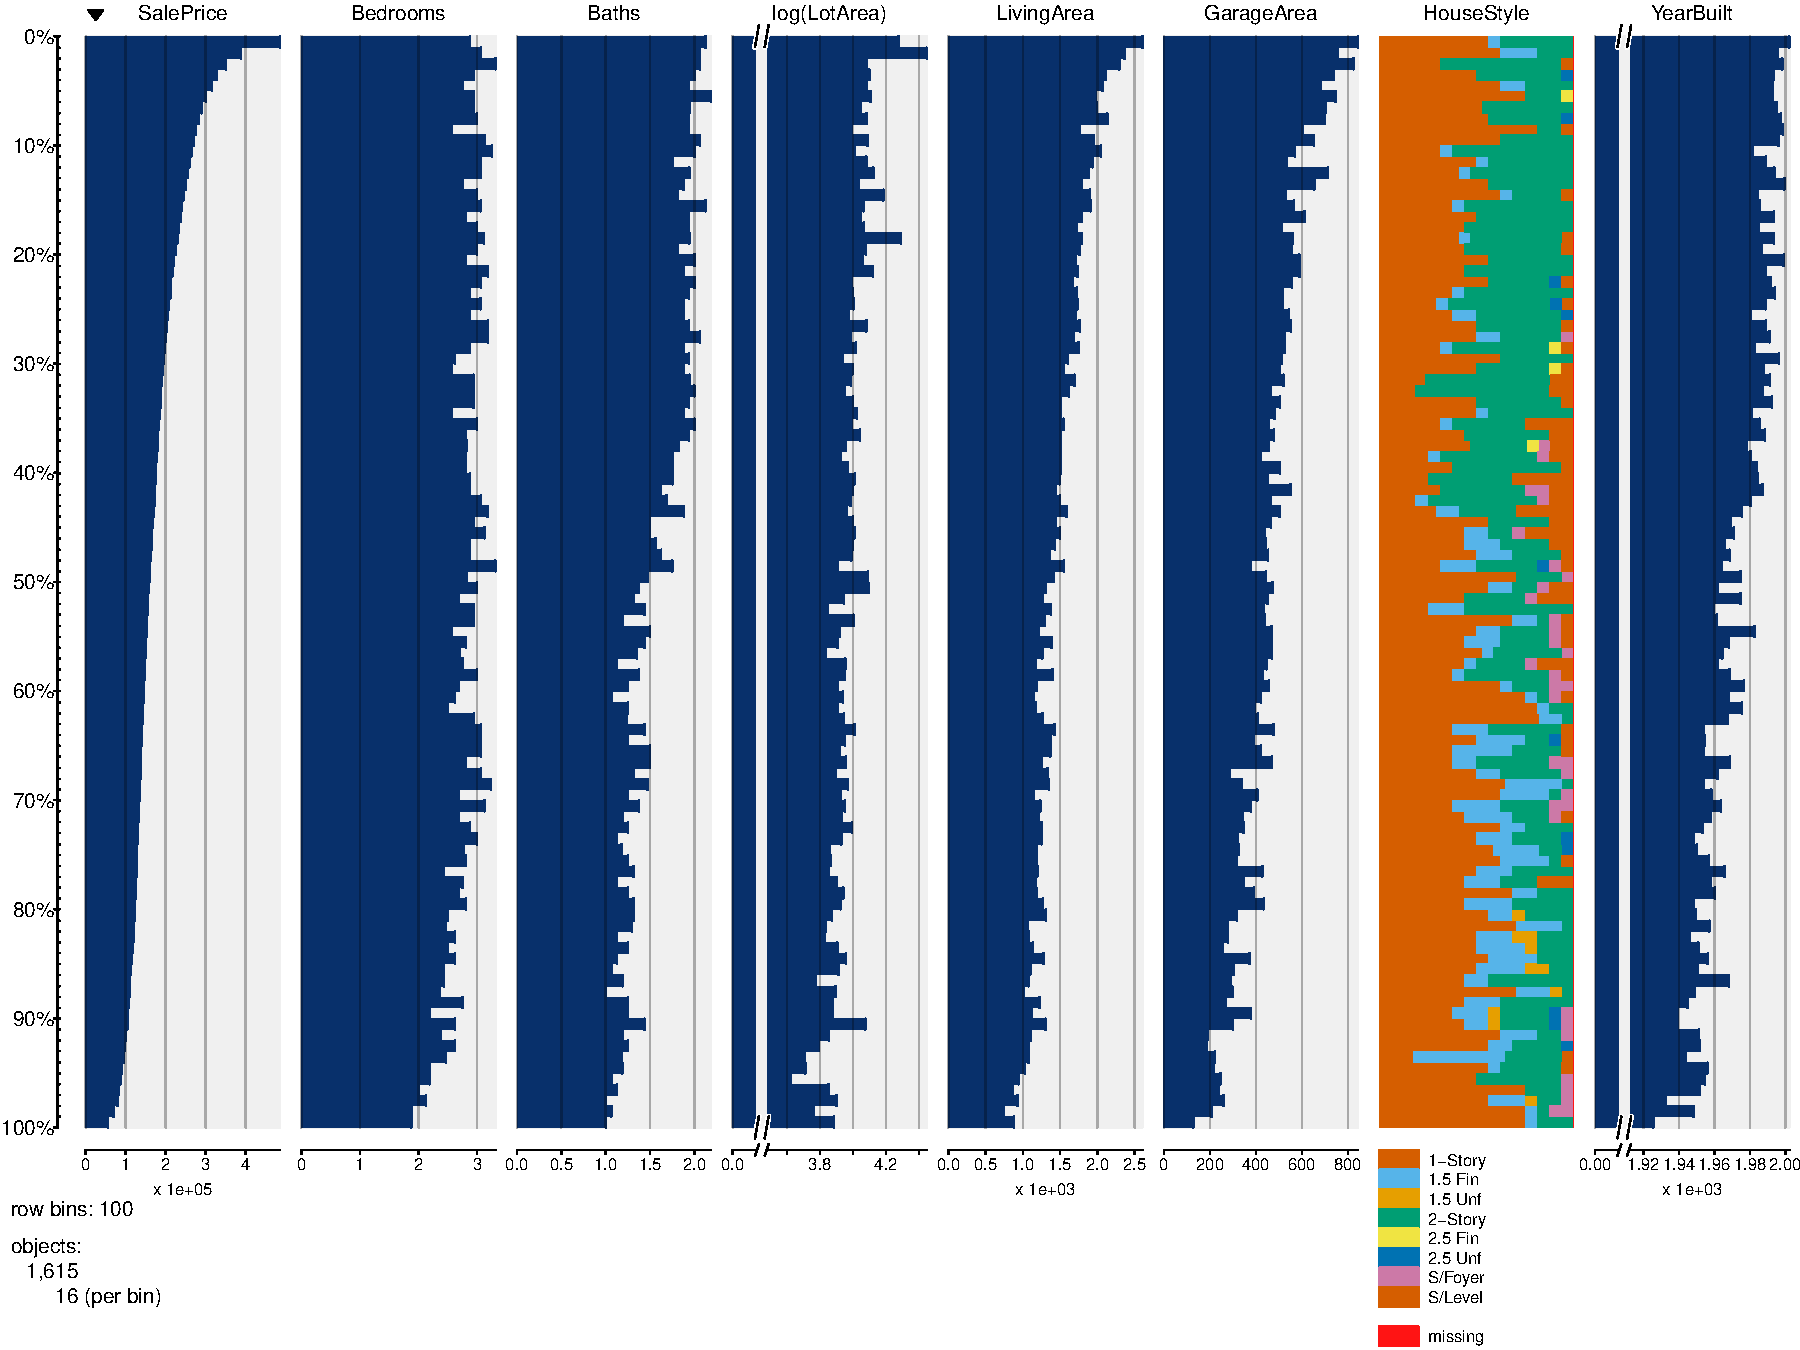
\includegraphics[width=0.95\textwidth]{images/tabplot.pdf}}
\caption{Table plot of Ames, Iowa, housing sales produced using the R package {\tt tabplot}. Variables that have a positive association have similarly shaped distribution.}
\label{tabplot}
\end{figure*}

Because the display uses a bar to represent mean values, there is implicit distortion of the data, a trait that is discouraged by \cite{Tufte83}. From a statistical perspective, we know that means or averages may not satisfactorily represent a set of numbers. Additionally, a mean is a point estimate, ideally represented by a point on a plot, with another graphical element, such as a line corresponding to standard error, displaying the variability associated with the estimate. Hence the table plot is a gross reduction and distortion of a large data set. to get a rough sense of the associations it may be reasonable to use, but it is ripe for re-designing to reduce data distortions, possibly by using dot displays \citep{Cl93}.

An interactive version of table plots is available with the R package {\tt tabplotd3} \citep{tabplotd3}. It uses the {\tt d3} software \citep{Bostock:2011} which is a javascript graphics library useful for creating interactive web visualizations.

\item Parallel coordinates

Another way to display high-dimensional data is the parallel coordinate plot \citep{In85,We90}. Several developments of these plots have been made in recent years. \citet{hurley.oldford} initially begin working on graphs as a way to organize the axes of a parallel coordinate plot, but the work has extended to provide an algorithm for navigating high-dimensional spaces. Their R package, {\tt PairsViz} \citep{pairviz}, implements the parallel coordinate plot style visualization. \citet{hofmann.vendettuoli} describe variations of parallel coordinate plots for categorical data and their R package, {\tt ggparallel} \citep{ggparallel}, enables others to use the methods. \citet{envelope} provide envelope methods for parallel coordinate plots for large data. 

\item Rearranging and summarizing data 

When data becomes very large an alternative approach can be to make summaries and display these. The {\tt ggplot2} package has revolutionized the display of data for many analysts, and it comes with siblings in the Wickham suite of software that can help process data for viewing in different ways: {\tt tidyr}, {\tt reshape2}, {\tt dplyr}, {\tt lubridate}, {\tt broom}, {\tt fstread}, {\tt bigrquery}, {\tt ggmap}, {\tt bigvis}.

The {\tt bigvis} package \citep{bigvis} summarizes large amounts of data using aggregation and smoothing techniques, and from these summaries users can make various plots with {\tt ggplot2}. Behind the {\tt plyr} \citep{plyr} and {\tt dplyr} \citep{dplyr} packages is the split-apply-combine strategy, meaning that the data is divided into chunks, a function is applied and the results are joined. For example, with climate records from multiple locations we might want to examine linear models at each location. This is easy to do with by split-apply-combine. The {\tt dplyr} package extends the approach with a grammar, and off-loads some computations to database operations.

The split-apply-combine strategy resembles the approach that hadoop \citep{hadoop} clusters employ for storing humongous data. Chunks of data are placed in different locations and indexed using keys. Accessing this data requires operating on chunks and combining the results. The Tessera project \citep{tessera} provides an R interface to hadoop style distributed file systems, and an early project paper \citep{guha} describes its use for visualizing large data. Another unpublished R package, {\tt iotools} \citep{urbanek} is available for pulling data from hadoop storage units.

%Instead of representing raw data with million points, sometimes it is better to summarize data in  proper way and use the summarized data for visualization. {\tt bigvis} \citep{bigvis}summarize big data using aggregation and smoothing techniques. It is very useful to use before plotting big data. After summarizing big data using{\tt bigvis}, the user can draw various plots using {\tt ggplot2}\citep{wickham2009ggplot2}. {\tt ggplot2} provides the easy way to generate complicated plots for exploring data analysis. It is developed under the grammar of graphics. It also provides multiple layers of plots that is useful to add statistical modeling results in the same plot.

\item Interactive graphics

This is still a work in progress, but there are some exciting developments. There have been many additional software tools (e.g. \citet{Bostock:2011}'s  {\tt D3}) available for interactive graphics, but close connections between these and statistical modeling, of the sort achieved in XLispStat \citep{Ti91}, is lagging. Some early explorations with interfaces in R were seen in \citet{iplots} which interfaced R with Java and \citet{rggobi-rnews} which interfaced R with C and gtk. Recent developments include {\tt cranvas} \citep{xie2014reactive}, {\tt ggvis} \citep{ggvis} and {\tt shiny} \citep{shiny}.  Cranvas provides interactive graphics inside R by using wrappers to qt graphics libraries, and hence theoretically can be used for really large data sets. GGvis provides web graphics using javascript, and shiny provides graphical user interface elements for the web. For python programmers, the library {\tt bokeh} \citep{bokeh} provides interactive web graphics using javascript.

\end{itemize}

%%%%%%%%%%%

Within the statistical literature there has been work on providing visual model diagnostics, a new plot type for visualizing clustering of multidimensional data and stronger connections between exploratory data analysis using graphics and inferential statistics. \citet{hofert2013graphical} provides a graphical goodness-to-fit test for dependence models in higher dimensions, and implements these in an R package, {\tt copula}. \citet{baddeley2013residual} provide new graphical residual diagnostics for covariate effects in spatial point processes, which help assess and improve the fit of these complex models. The R package, {\tt spatstat}, is extended to incorporate these diagnostics. Rainbow plots and bagplots \citep{rainbow} were developed for viewing a large number of functional data, smooth curves or surfaces, and has an accompanying R package. \citet{van2011visualizing} propose the visualization method for a hierarchical tree of high density clusters in high dimensional data. They project the multidimensional clusters to a 2D or 3D layout using an optimized star coordinates layout. It allows to explore the distribution of clusters interactively and helps the user to understand the relationship between the clusters and the original data space. \citet{newell} describe methods for finding clusters in populations based on genetic markers, very sparse, high-dimensional data, and using the tour \cite{As85} to visualize the cluster structure. \citet{buja:2009} and \citet{majumder:2013} detail new protocols for data visualization that would enable statistical inference to be conducted to quantify the significance of structure seen in plots. This is really important development for working with big data sets, because we typically do not have a classical inference environment. It is easy to imagine patterns in data, and these protocols provide a way to determine if what we see is really there. As a statistician, strictly adhering to the rigid assumptions required by classical hypothesis testing, runs the risk of non-discovery, failing to see something that is present in the data. This new work makes it possible for statisticians to be both explorers and skeptics. The protocols are implemented in the R package {\tt nullabor} \citep{nullabor}.  

% Massively Parallel Nonparametric Regression, With an Application to Developmental Brain Mapping 23(1) 2014
%Philip T. Reiss, Lei Huang, Yin-Hsiu Chen, Lan Huo, Thaddeus Tarpey and Maarten Mennes

%When the number of dependent variables are very large and we need to model them with same covariates, the computational burden increases enormousyl, especially when we need to consider the penalty term with the tuning parameter. \citet{reiss2014massively} proposed  the efficient algorithm for massively parallel nonparametric regression.  Also they suggested the way to summarize the significant models from nonparametric regression using clustering method. With these clusters, the user can easily figure out models with similar patterns. It is very helpful for dependent data in very high dimensional space, especially for the spatial type-dependency data for example, neuroimaging data. This method is provided as R package {\tt vows}.

In the infovis community there have been many developments for working with large data sets. OnSet\citep{sadana2014onset} is a technique to visualize large-scale binary set data. One observation is represented in one layer of plot and one pixel represents one elements in the plot. For the elements in this observation, pixels are highlighted. With these type of representation, it is easy to compare data sets using boolean operations. \citet{nanocubes} makes it easy to slice and dice large spatiotemporal data sets for viewing in various ways. 

The biological community has been grappling with humongous data sets for many years. There is still consderable work to be done to provide better visualization for these volumes of data but there are some exciting recent developments. The software epivizr \citep{epivizr} provides interactive web graphics, produced with javascript, closely linked with analysis tools available in R from the bioconductor suite. 

%\section{Technological Advances}

%\begin{itemize}
%	\item{Scalable computing system}
	
%	Hadoop file system (HDFS) and map reduce methods allow manipulation of big data in finite time making EDA possible in real time which otherwise is hard to achieve. For this statistical software R can be used with HDFS and high quality graphics can be produced in real time. I (Mahbub) will write in this direction and can put some references if you think something like this would be useful.......
	
%\end{itemize}

\section{Synopsis}

\citet{gelman2013infovis}, a featured article in the Journal of Computational and Graphical Statistics, with invited commentary, wrestles with the relative roles and purposes of statistical graphics and information visualization. It would be useful for scientists to have a taxonomy of nomenclature related to data visualization. Unfortunately, this article falls short. The invited commentaries do a nice job of defusing the incense provoked by the simplistic interpretation of these two areas of data visualization, where the differences are reduced to a matter of appearance vs functionality. 

There are many different names associated with data visualization: statistical graphics, information visualization, visual analytics, infographics. A taxonomy of the nomenclature is imperfect, the roles, purposes and functionality overlap, and the borders are porous. However, the existence of different terms indicates that there are useful, if not important, distinctions between them. Statistical graphics does have a primary focus of visualization of data associated with understanding variability. It can be elegant, interactive, and beautifully crafted. A lot of the time, though, it is ephemeral, designed to support to activity of exploratory data analysis.   

Explain working definitions of terms related to data visualization: infographics, information visualization, visual analytics

Talk about fishing! And avoiding fishing. And Buja's post-model ...


\bibliographystyle{asa}
\bibliography{visualization}

\end{document}

% John Deere, Andy Roberts

% Data Mining Cup team

% Phil Brierley


